\section{\texorpdfstring{Resolución de la ecuación \(f(x) = x^4 - 5x^2 - 2x + 1\) por medio de la Serie de Fourier}{Resolución de la ecuación f(x) = x\string^4 - 5x\string^2 - 2x + 1 por medio de la Serie de Fourier}}
\subsection{Braulio Gael Porras Zuñiga}

\begin{figure}[H]
	\centering
	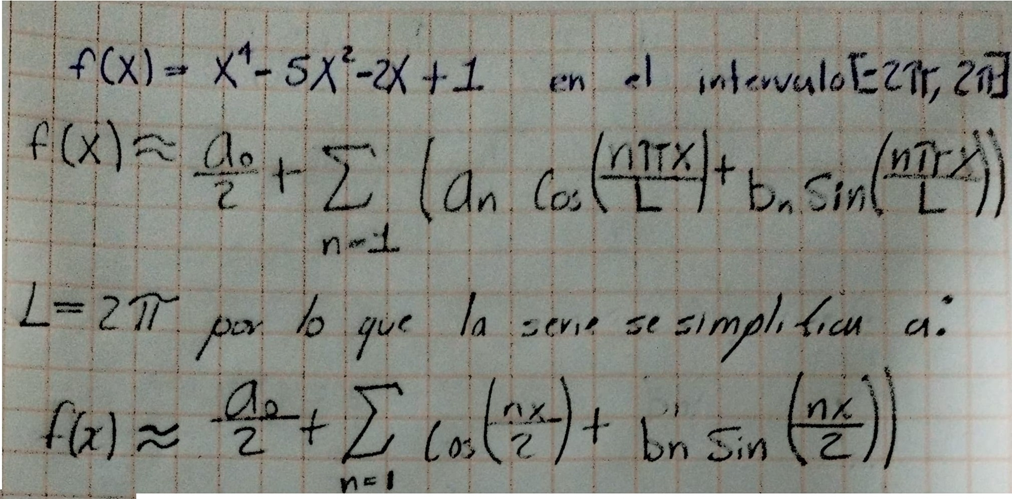
\includegraphics[width=5.15104in,height=2.54129in]{media/image52.png}
	\caption{Imagen 1A. Procedimiento de Fourier}
\end{figure}

\begin{figure}[H]
	\centering
	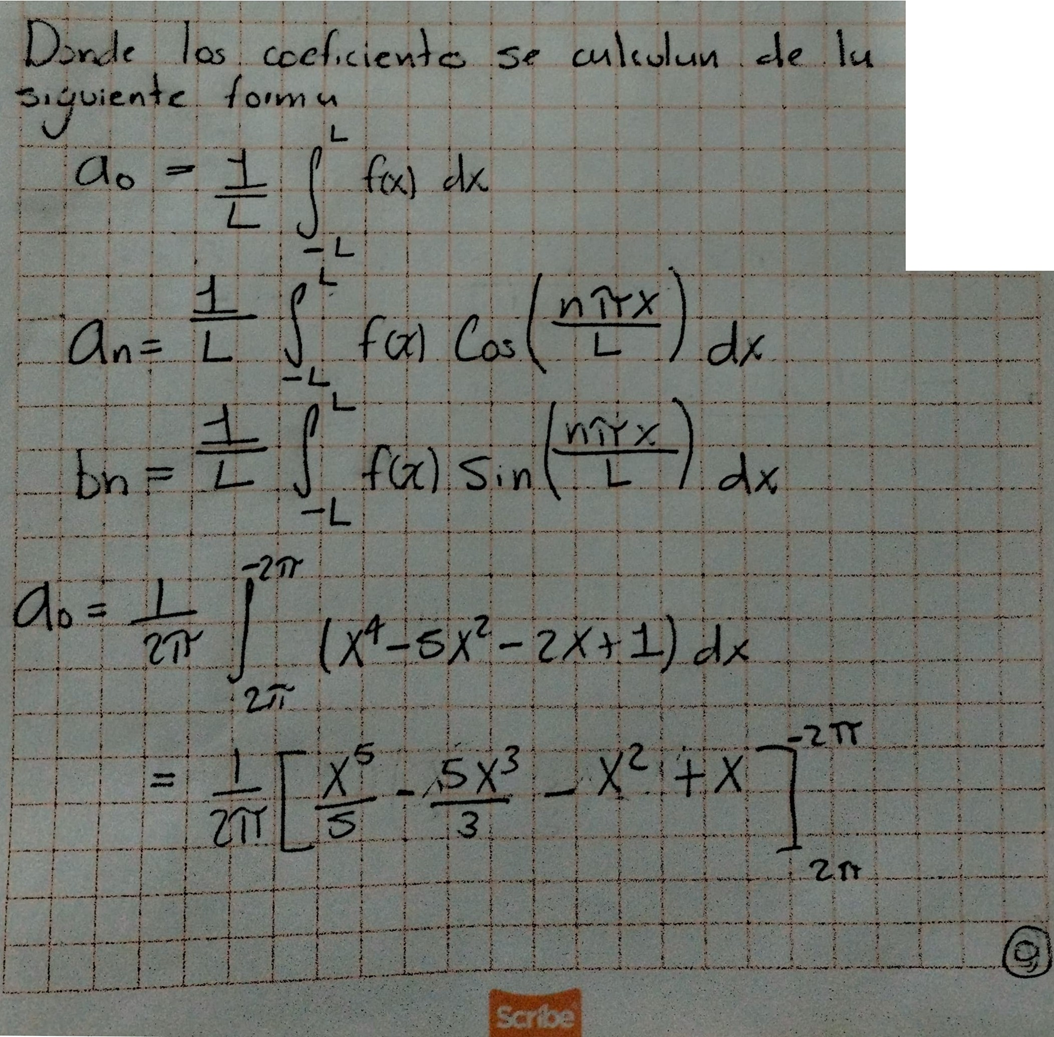
\includegraphics[width=3.66667in,height=3.60643in]{media/image49.png}
	\caption{Imagen 2A. Procedimiento de Fourier}
\end{figure}

\begin{figure}[H]
	\centering
	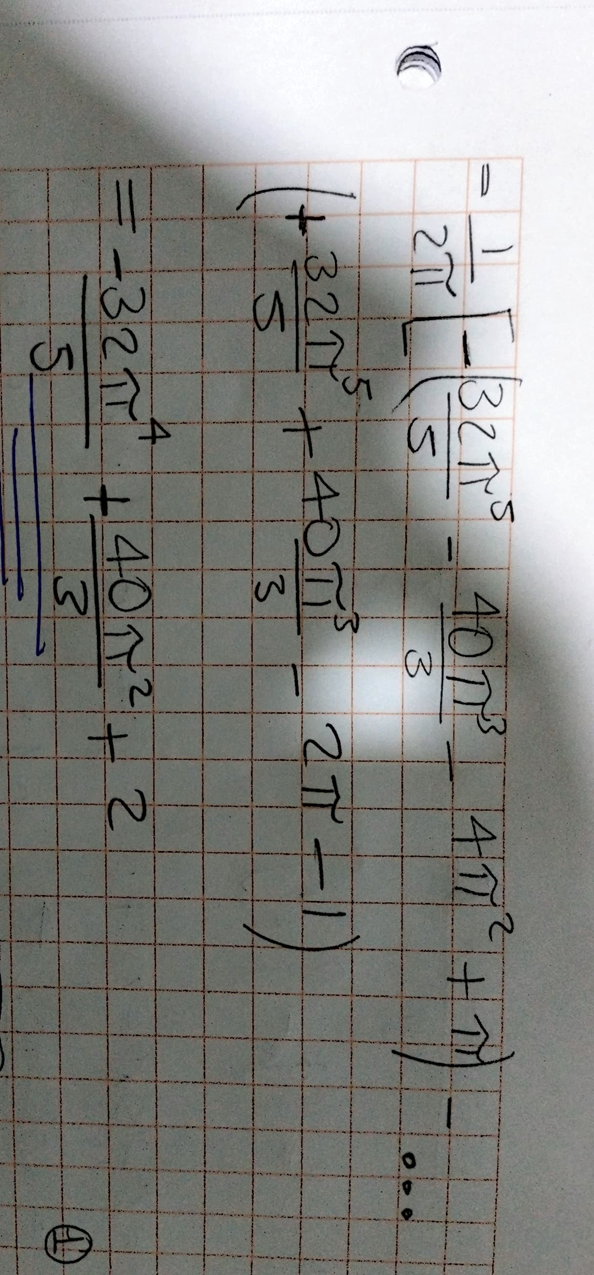
\includegraphics[width=2.34606in,height=5.02604in]{media/image54.png}
	\caption{Imagen 3A. Procedimiento de Fourier}
\end{figure}

\begin{figure}[H]
	\centering
	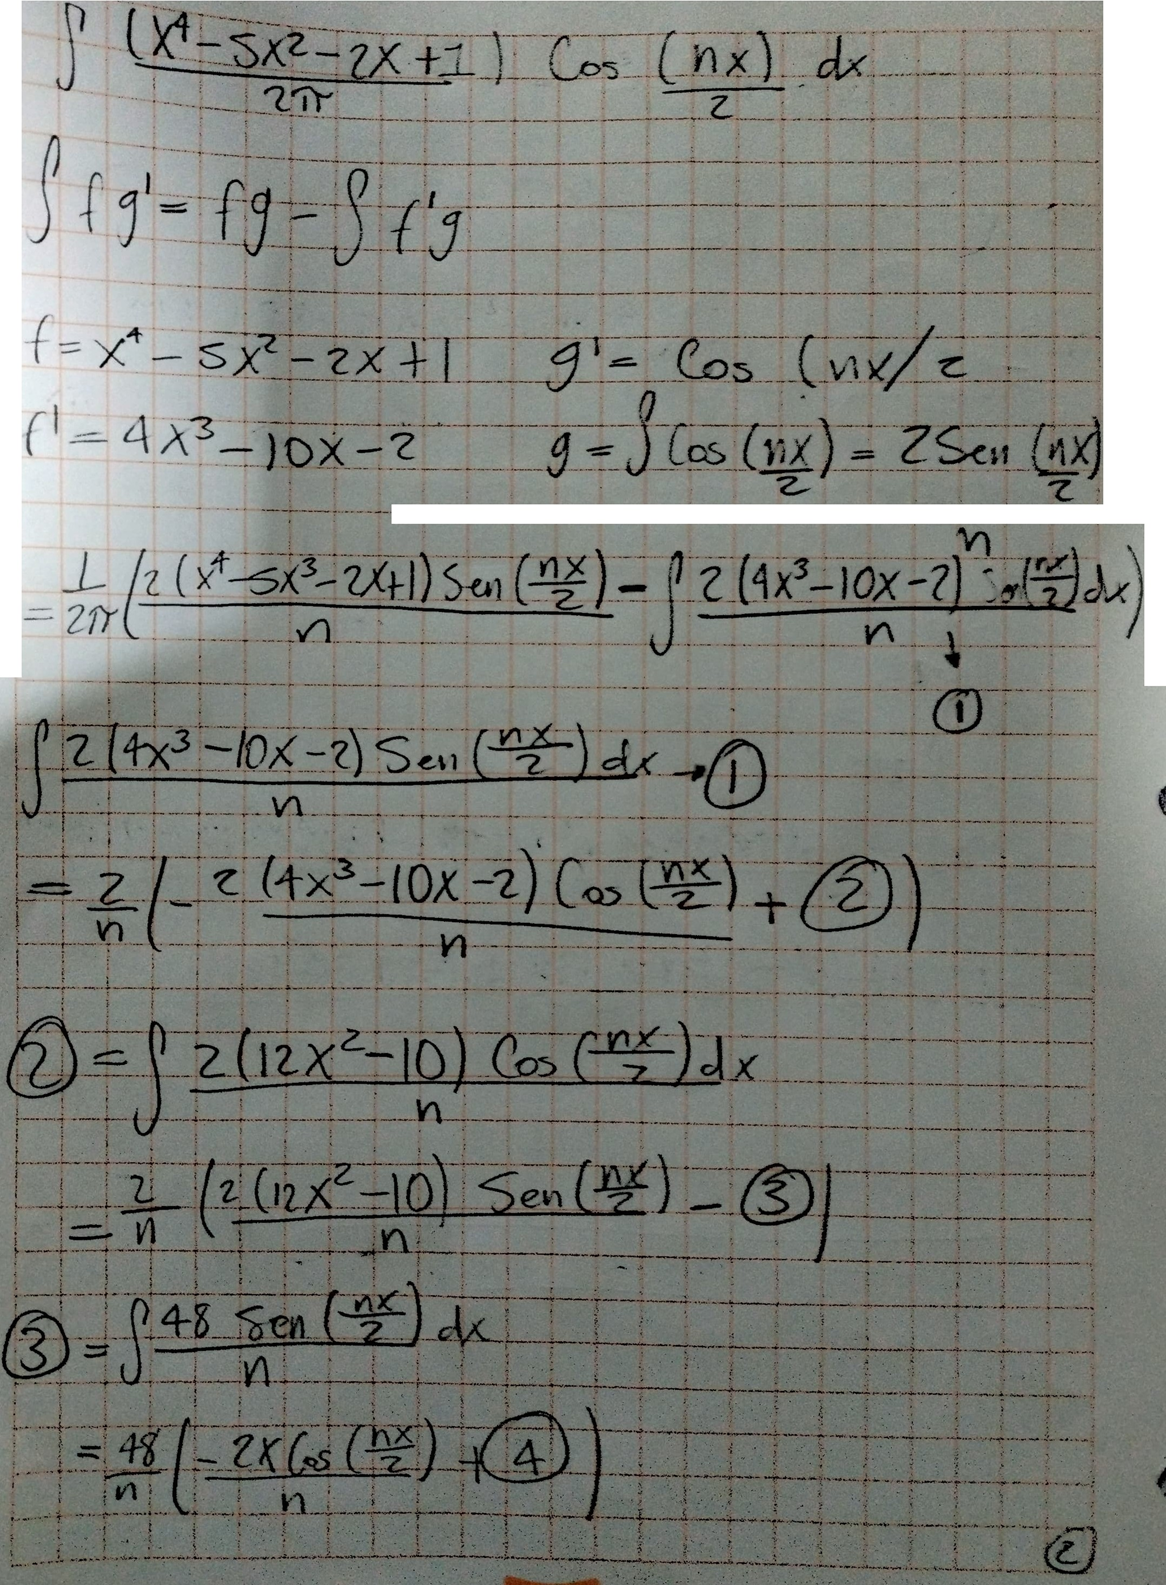
\includegraphics[width=4.84817in,height=6.58854in]{media/image48.png}
	\caption{Imagen 4A. Procedimiento de Fourier}
\end{figure}

\begin{figure}[H]
	\centering
	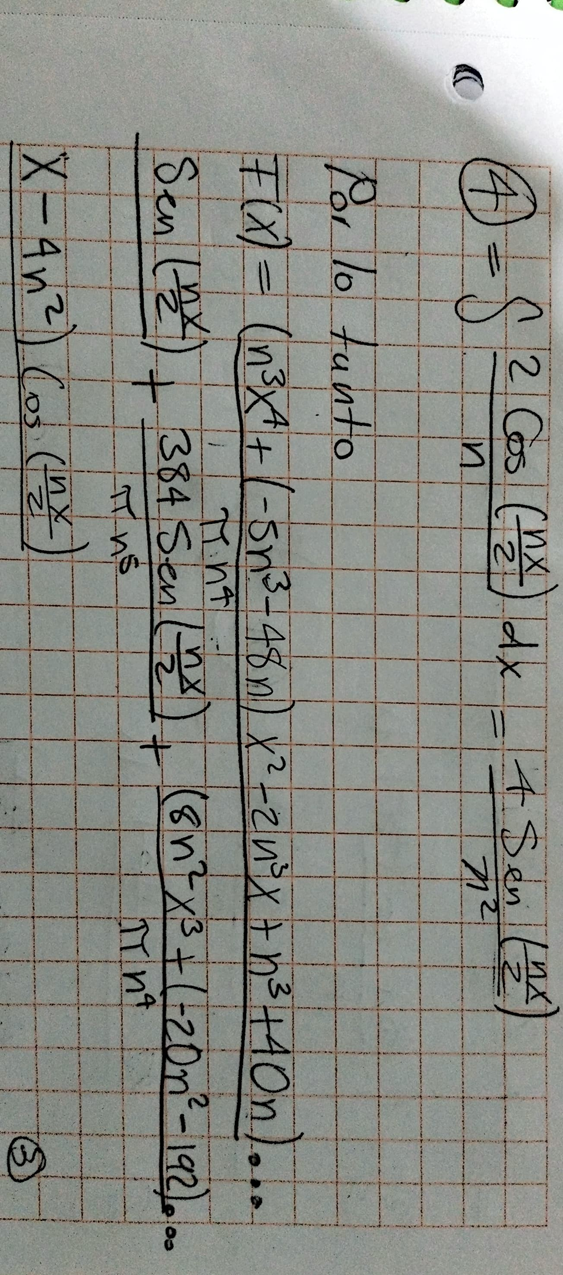
\includegraphics[width=2.15104in,height=4.88023in]{media/image22.png}
	\caption{Imagen 5A. Procedimiento de Fourier}
\end{figure}

\begin{figure}[H]
	\centering
	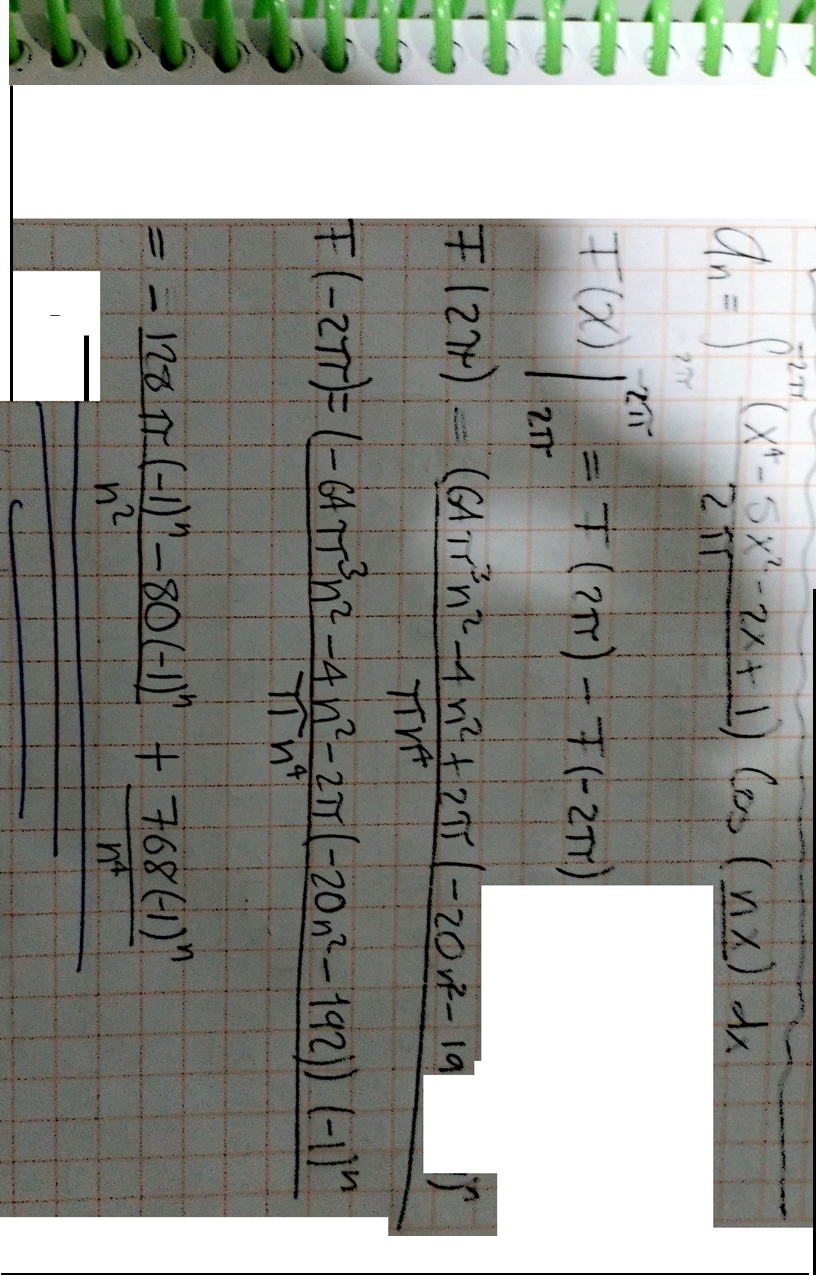
\includegraphics[width=3.07924in,height=4.81771in]{media/image51.png}
	\caption{Imagen 6A. Procedimiento de Fourier}
\end{figure}

\begin{figure}[H]
	\centering
	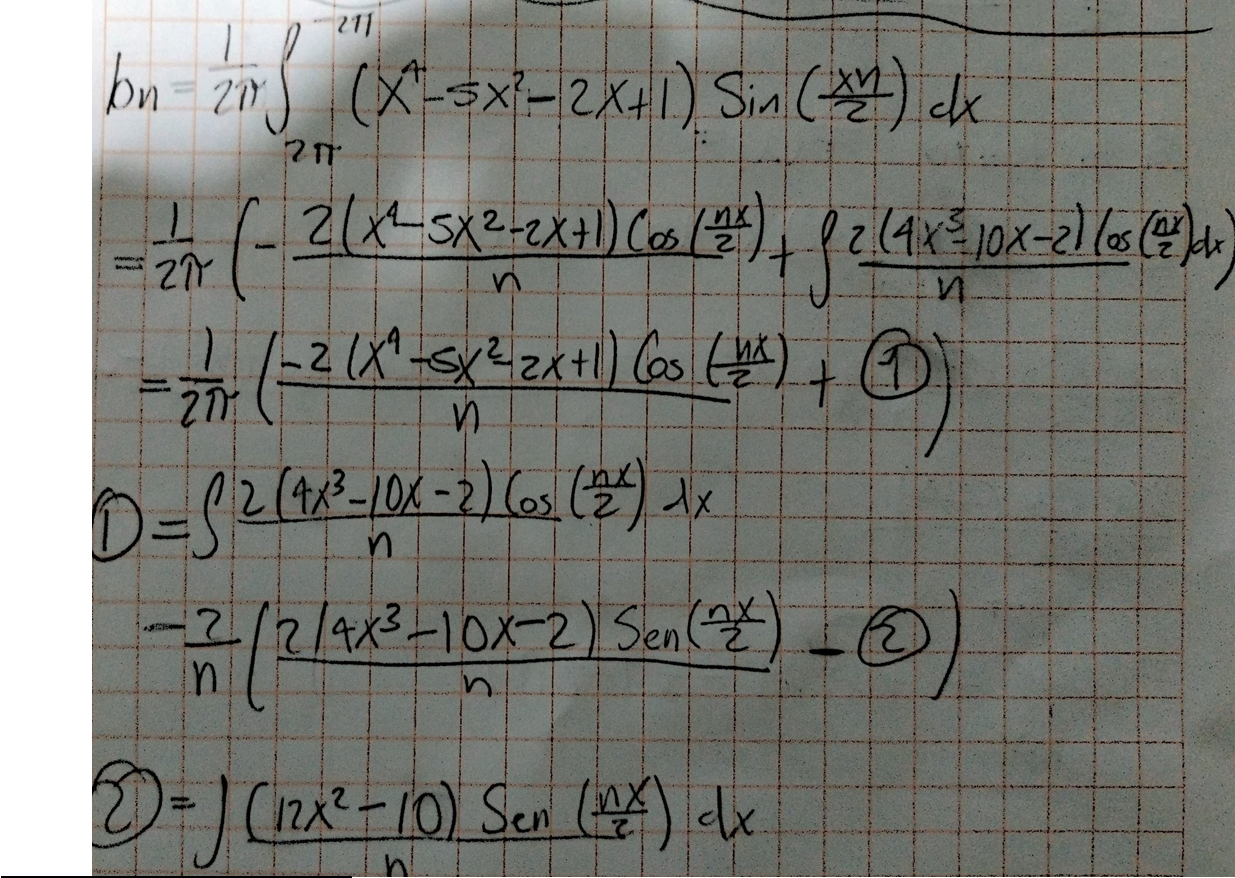
\includegraphics[width=4.74479in,height=3.37337in]{media/image47.png}
	\caption{Imagen 7A. Procedimiento de Fourier}
\end{figure}

\begin{figure}[H]
	\centering
	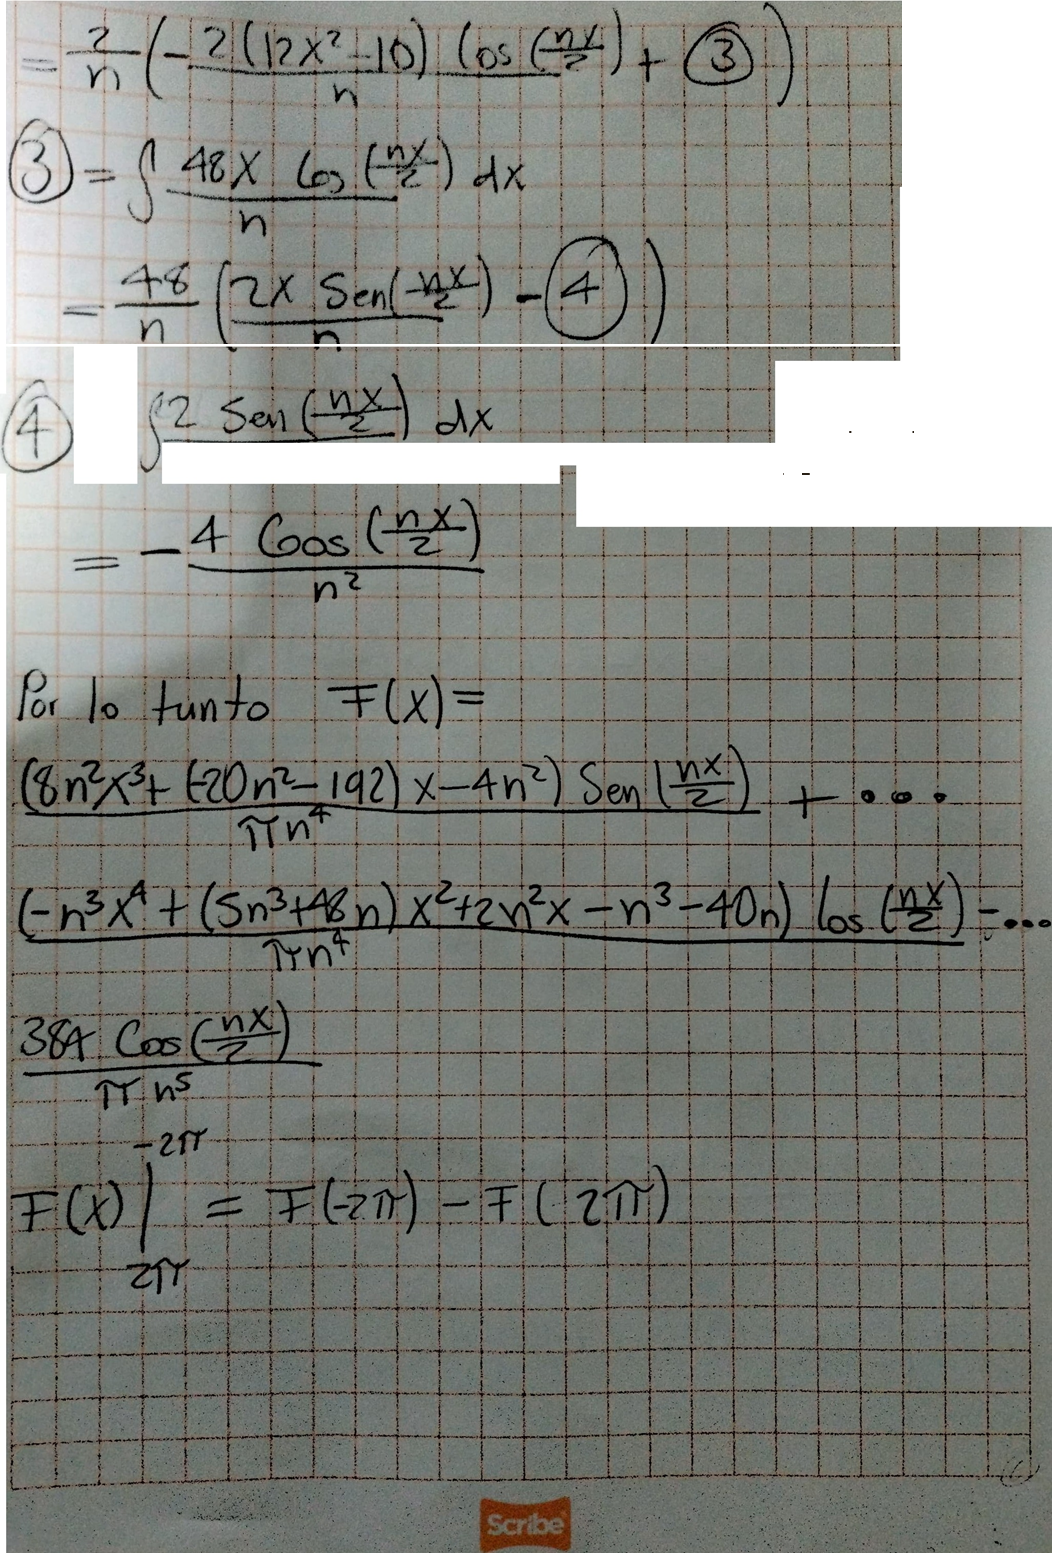
\includegraphics[width=4.94271in,height=7.29091in]{media/image53.png}
	\caption{Imagen 8A. Procedimiento de Fourier}
\end{figure}

\begin{figure}[H]
	\centering
	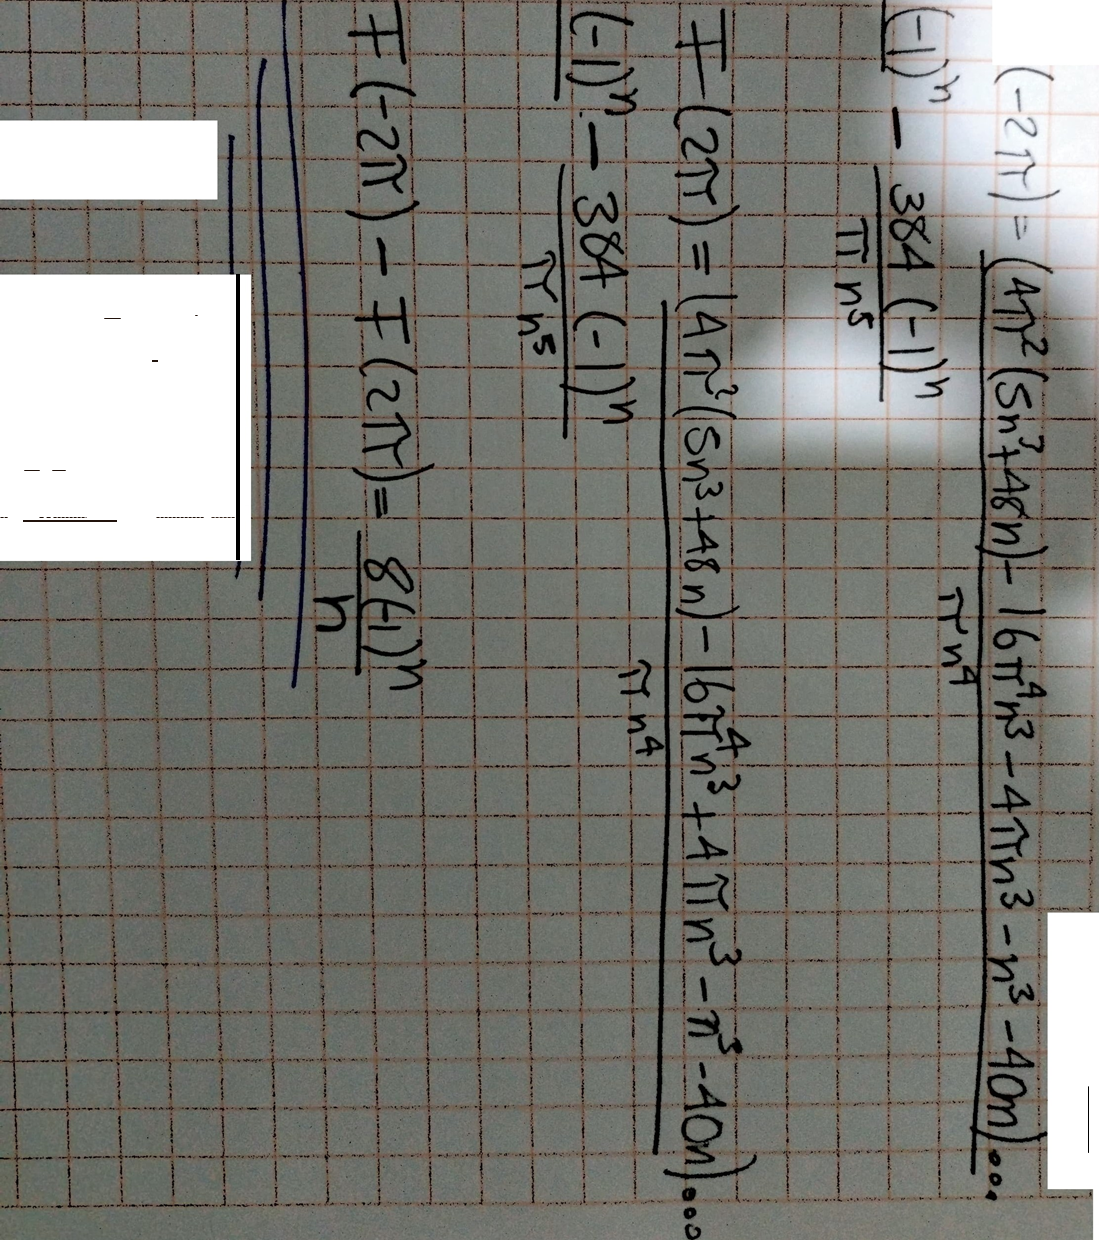
\includegraphics[width=3.88021in,height=4.37099in]{media/image43.png}
	\caption{Imagen 9A. Procedimiento de Fourier}
\end{figure}

\subsection{Magaly Citlali Jimeno Reyes}

\begin{figure}[H]
	\centering
	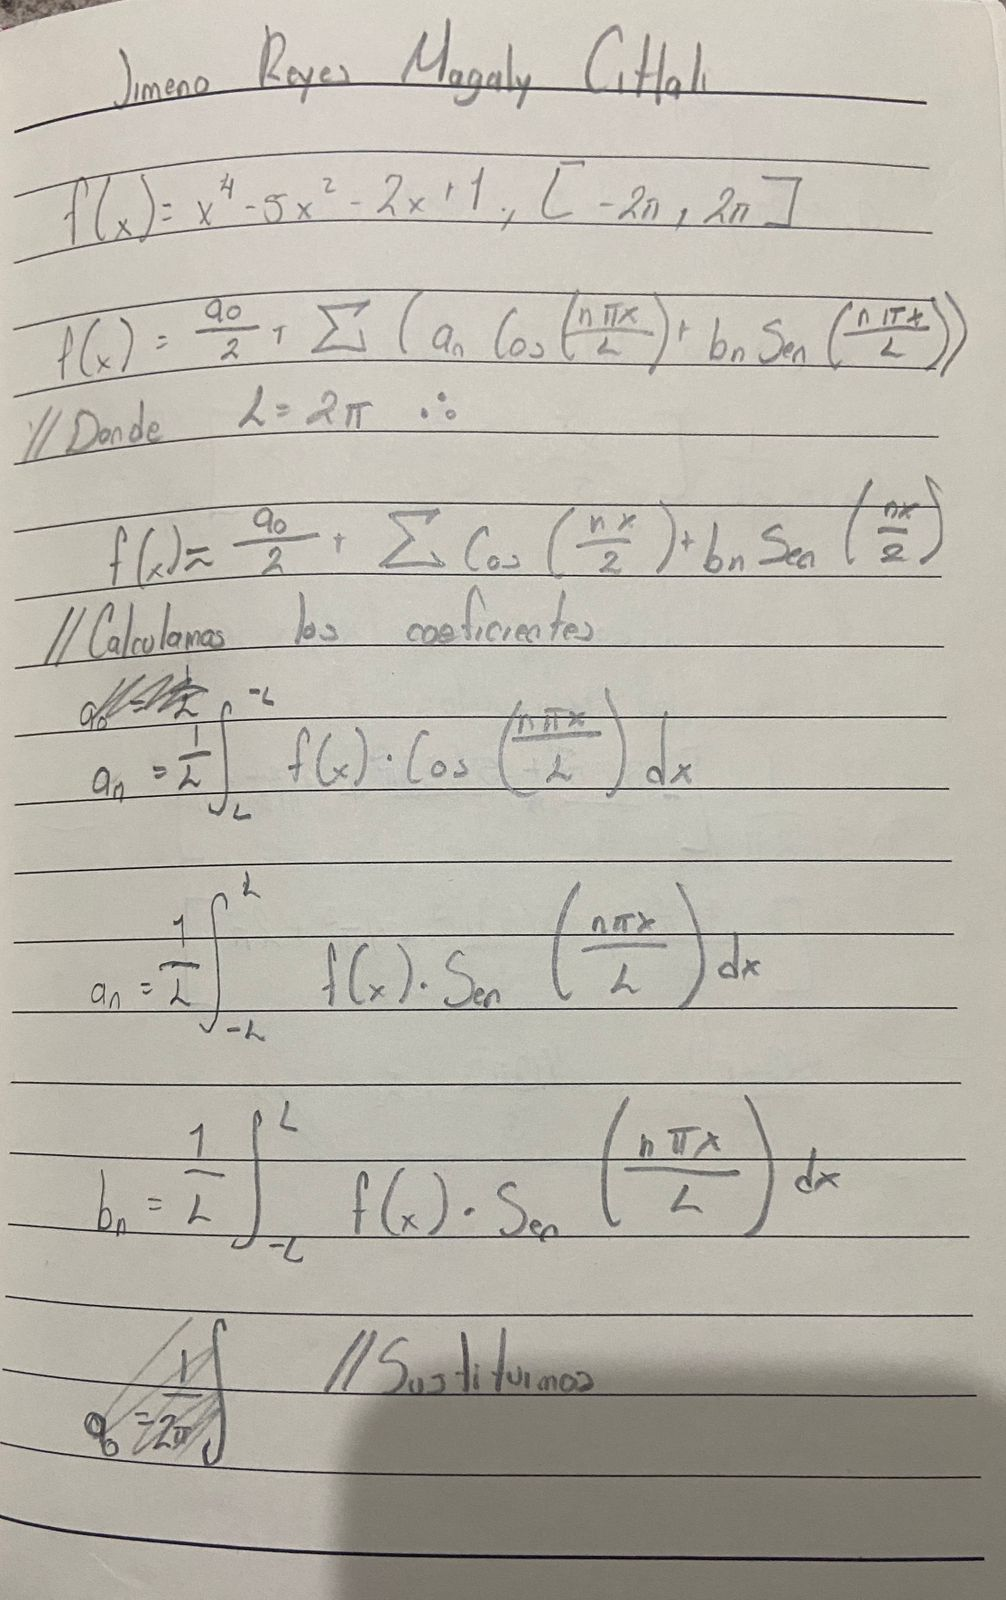
\includegraphics[width=2.98958in,height=4.74434in]{media/image13.jpg}
	\caption{Imagen 1B. Procedimiento de Fourier}
\end{figure}

\begin{figure}[H]
	\centering
	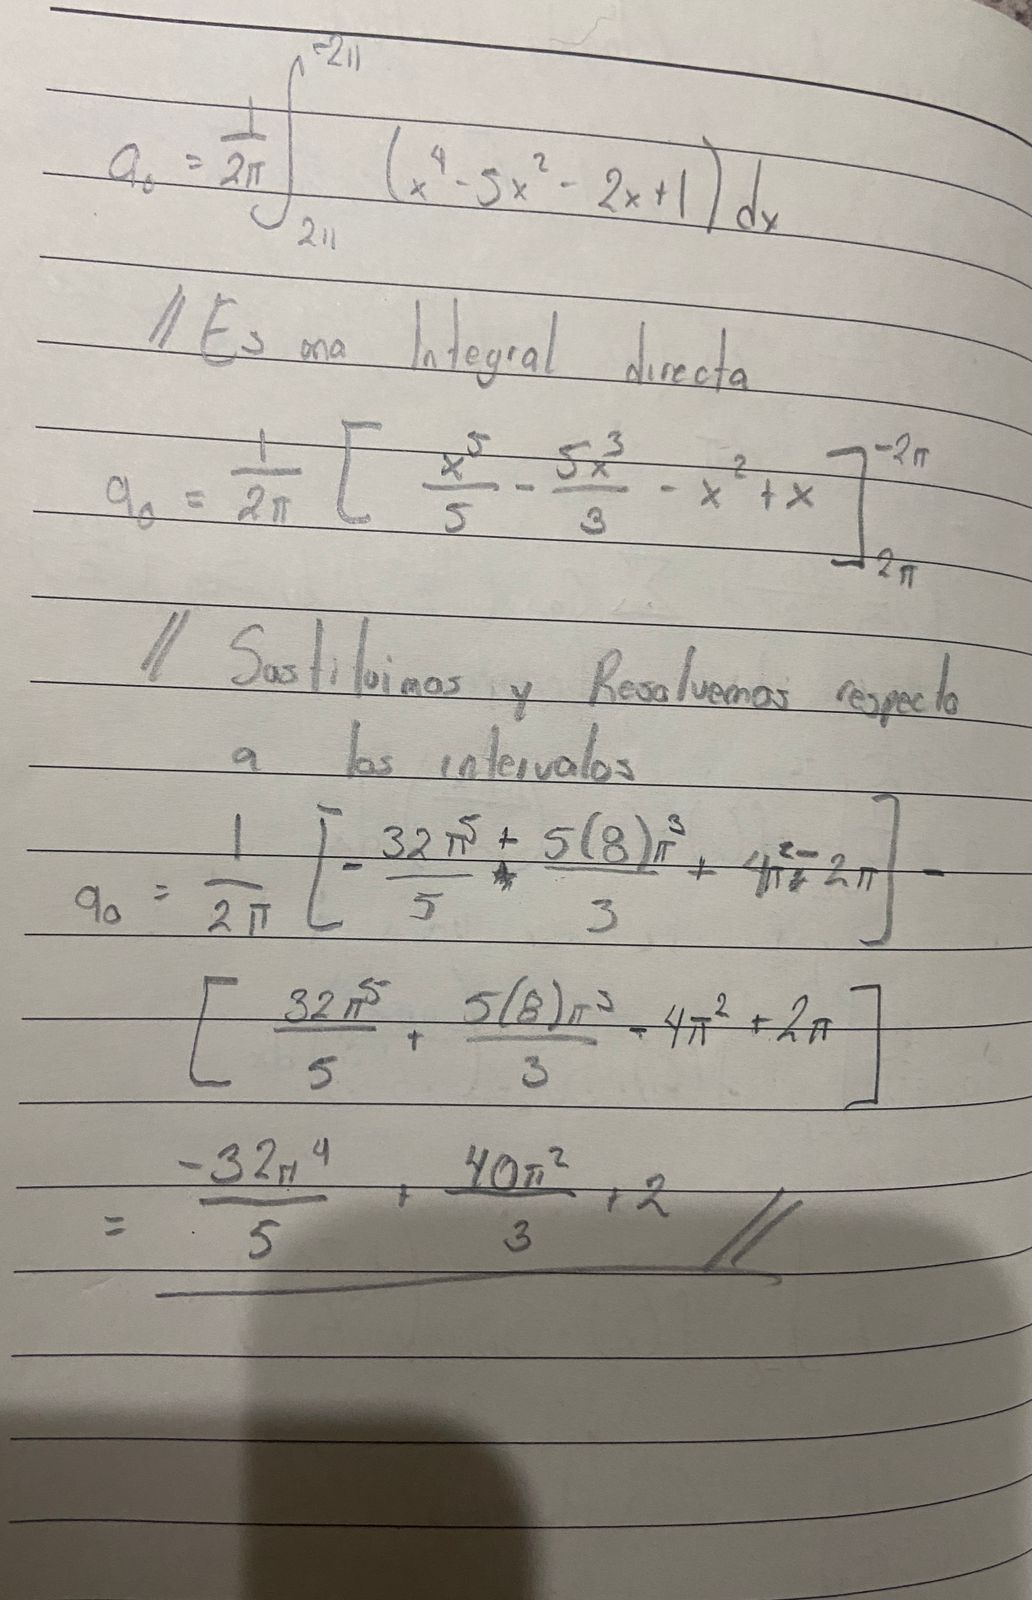
\includegraphics[width=3.03622in,height=4.74409in]{media/image8.jpg}
	\caption{Imagen 2B. Procedimiento de Fourier}
\end{figure}

\begin{figure}[H]
	\centering
	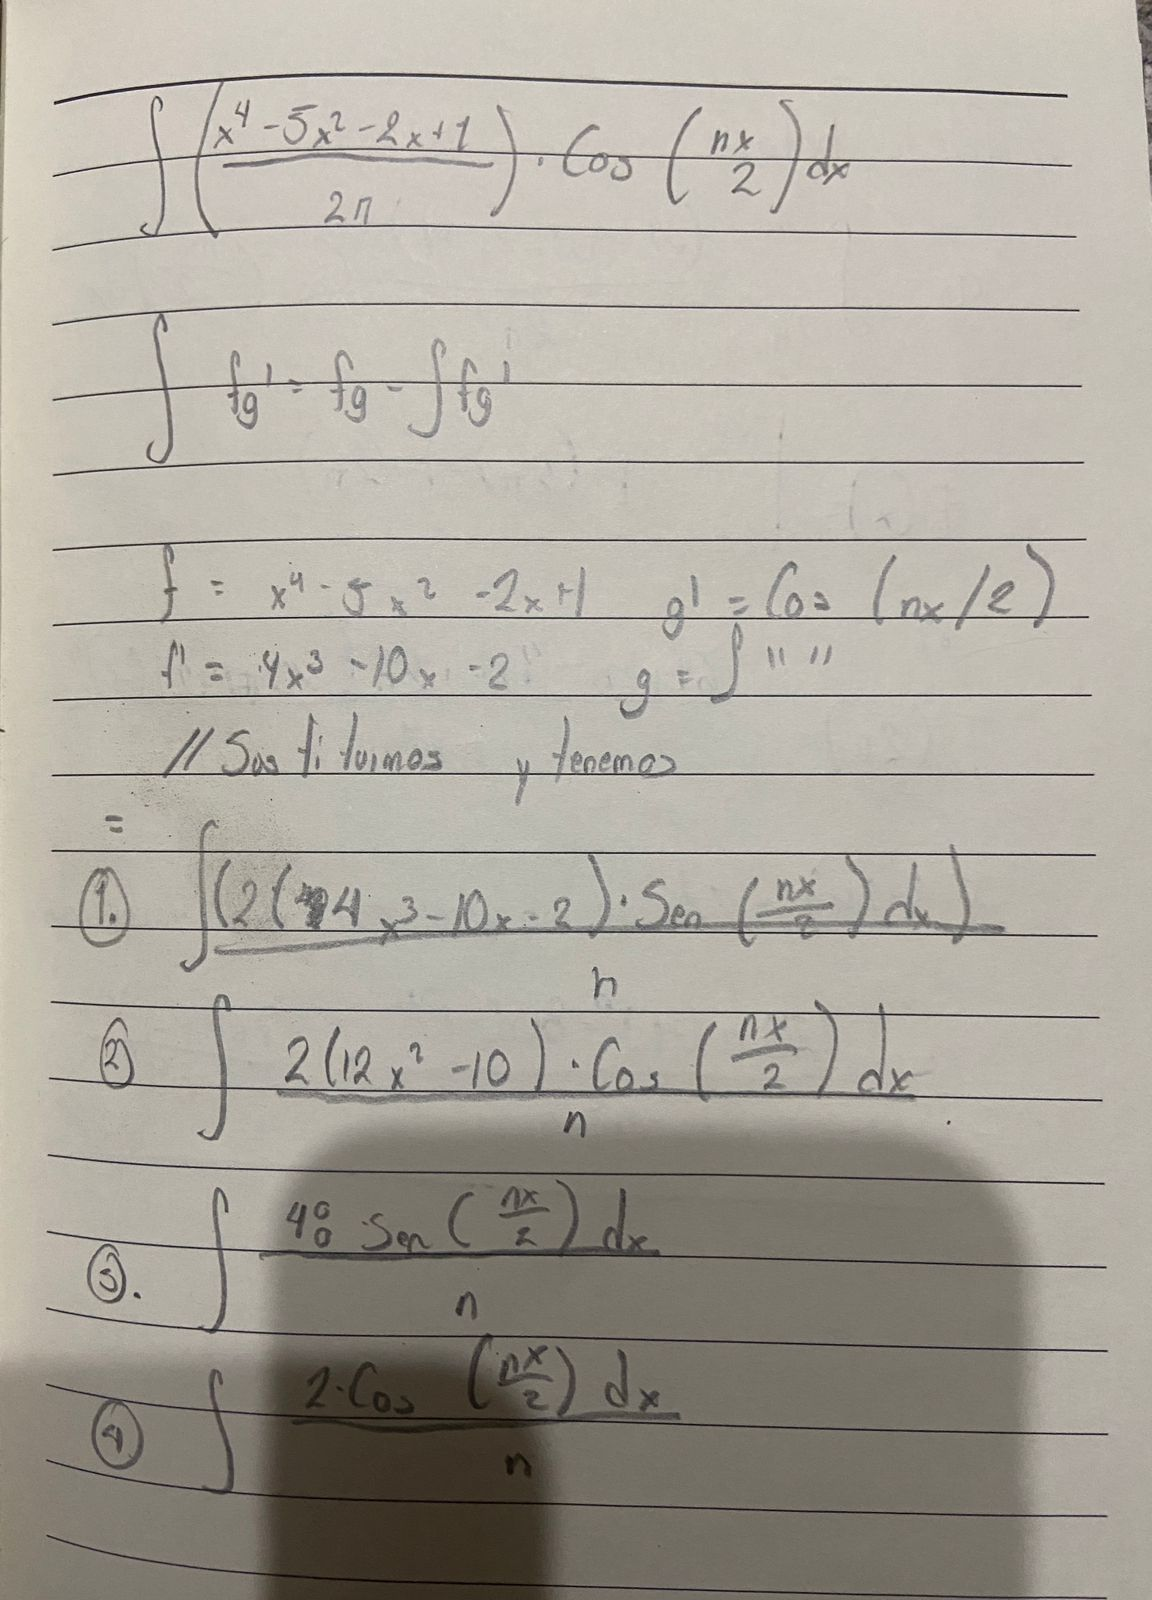
\includegraphics[width=3.0625in,height=5.18146in]{media/image42.jpg}
	\caption{Imagen 3B. Procedimiento de Fourier}
\end{figure}

\begin{figure}[H]
	\centering
	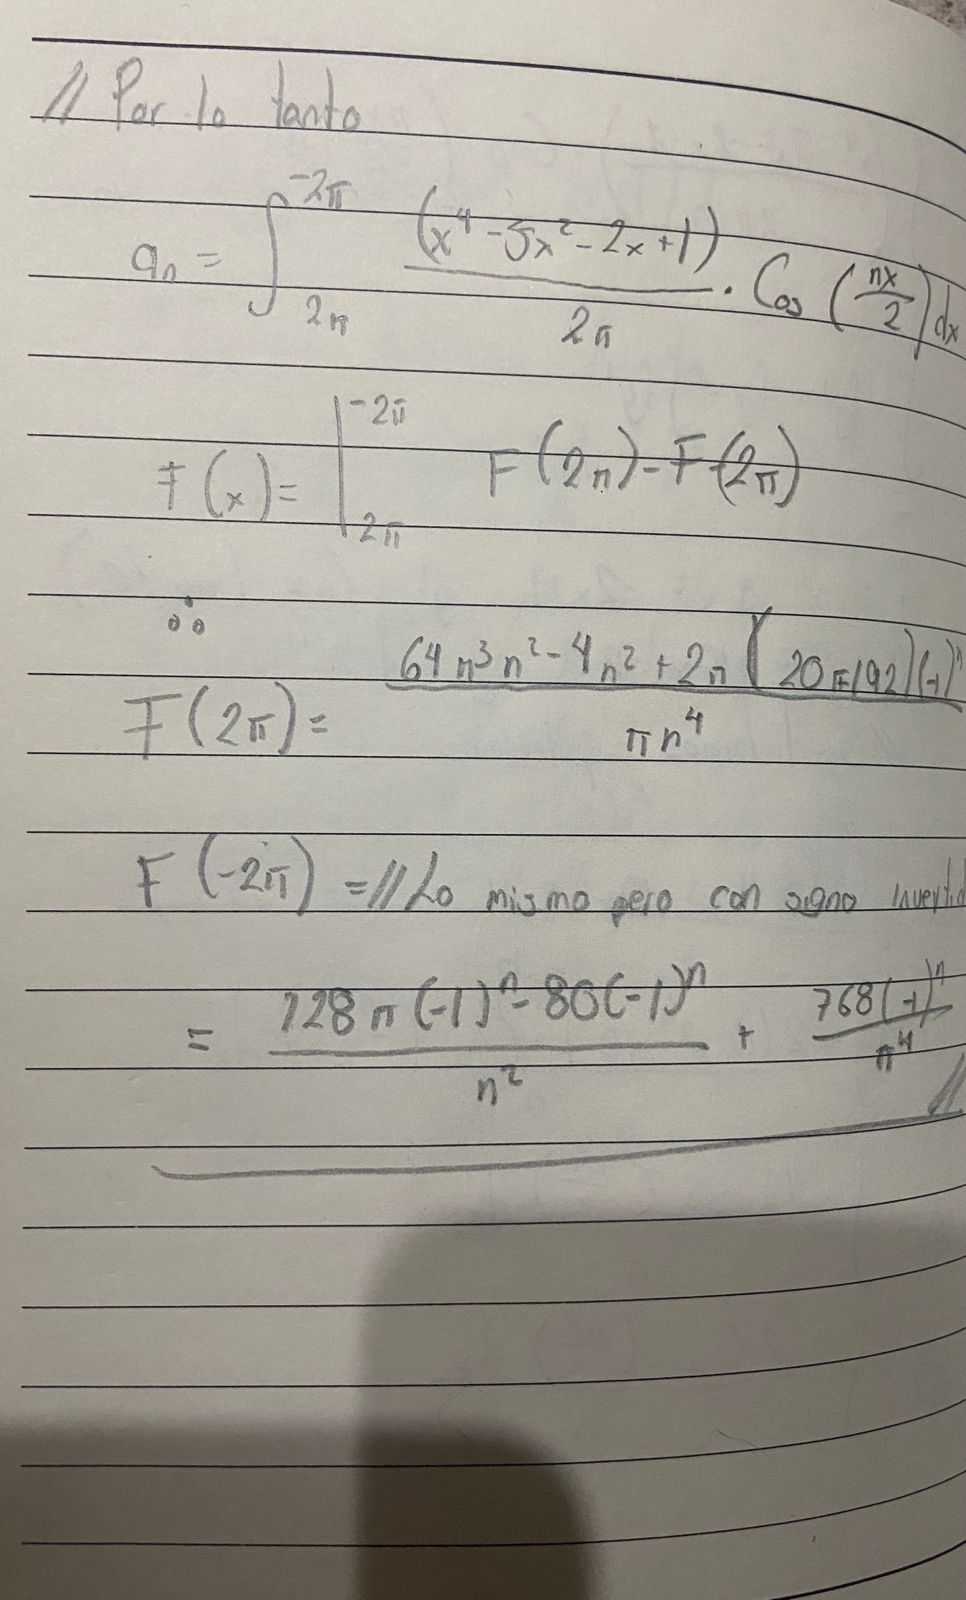
\includegraphics[width=2.97297in,height=4.92052in]{media/image2.jpg}
	\caption{Imagen 4B. Procedimiento de Fourier}
\end{figure}

\begin{figure}[H]
	\centering
	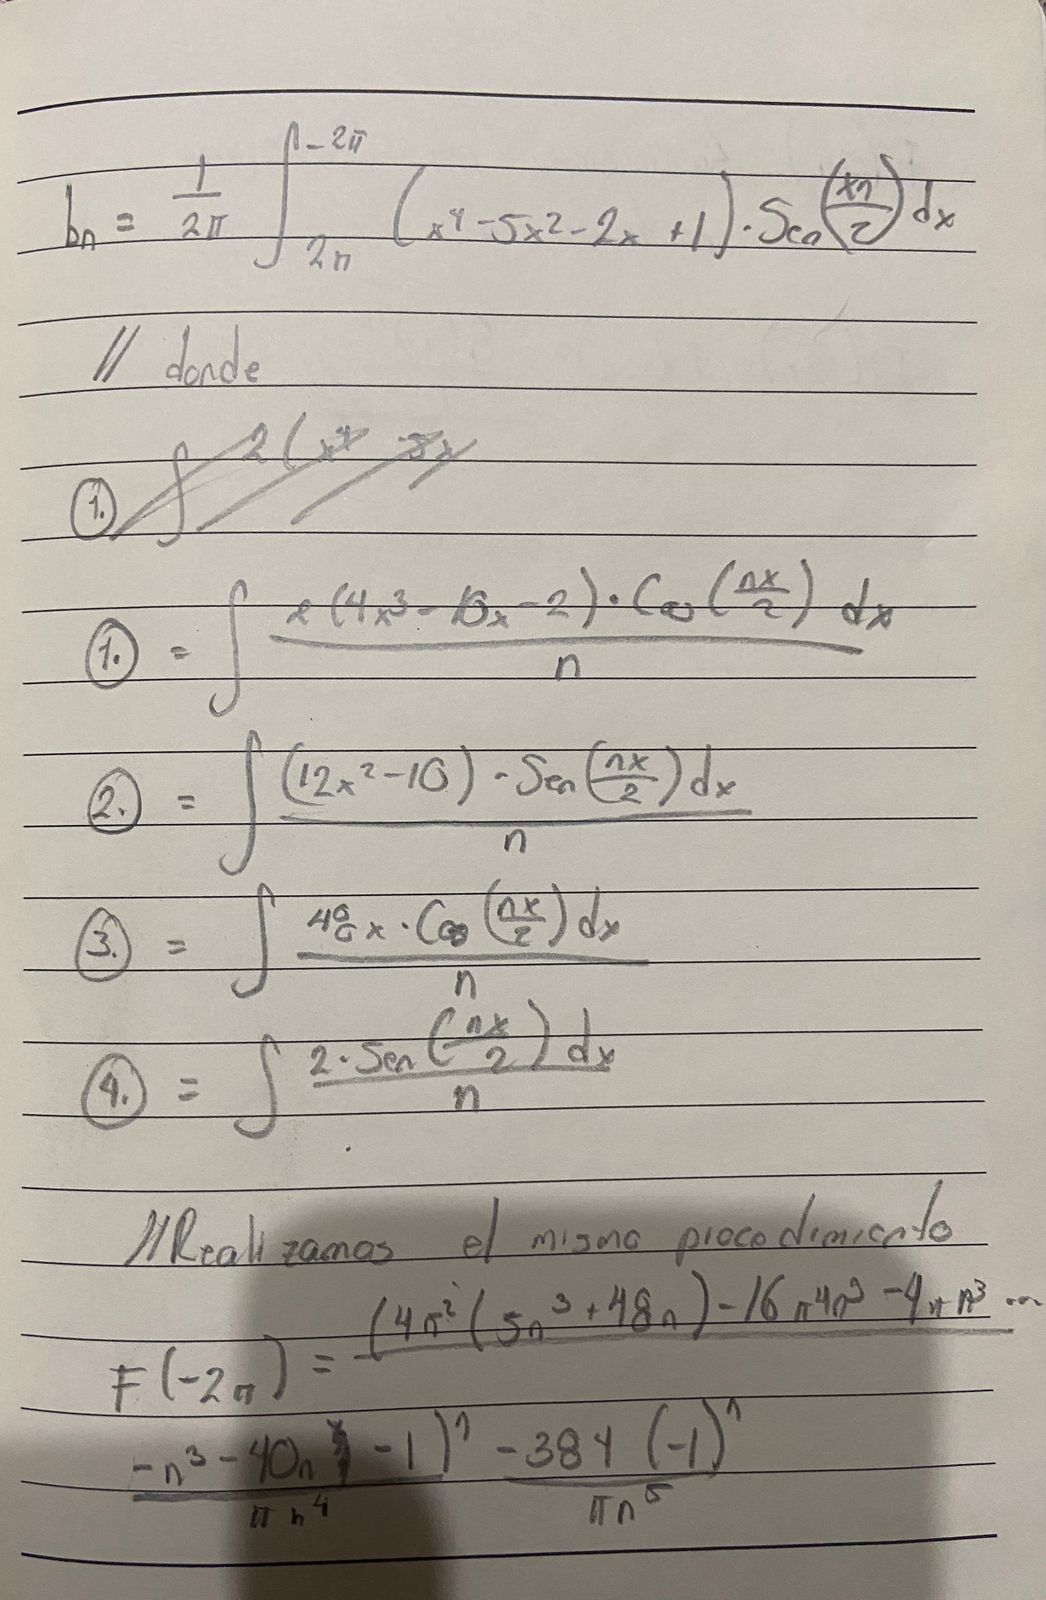
\includegraphics[width=3.1436in,height=4.80787in]{media/image9.jpg}
	\caption{Imagen 5B. Procedimiento de Fourier}
\end{figure}

\begin{figure}[H]
	\centering
	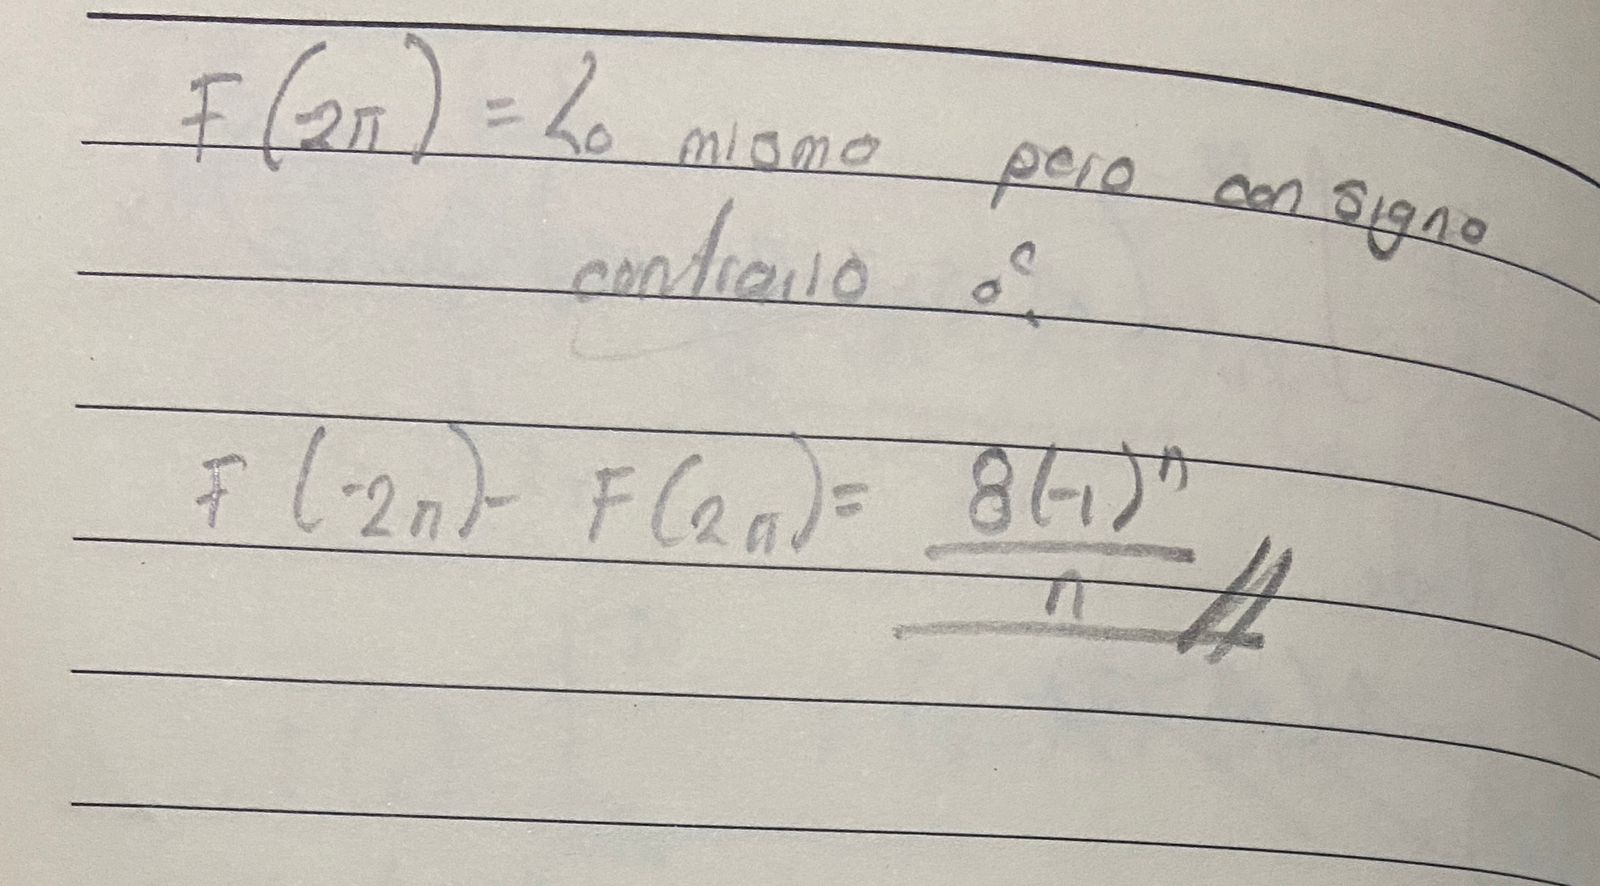
\includegraphics[width=3.00684in,height=3.1593in]{media/image46.jpg}
	\caption{Imagen 6B. Procedimiento de Fourier}
\end{figure}

\subsection{Juárez Botello Josué Adalid}

\begin{figure}[H]
	\centering
	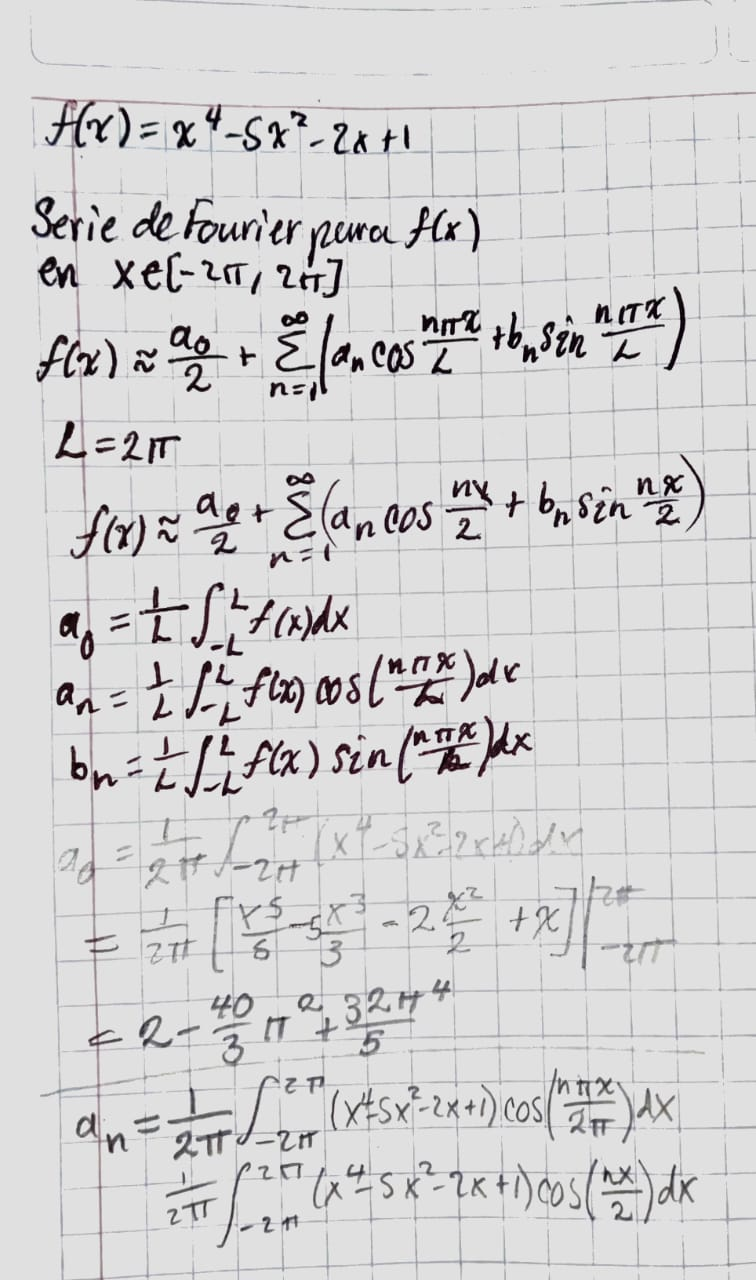
\includegraphics[width=3.19696in,height=5.41146in]{media/image44.jpg}
	\caption{Imagen C1. Primero, establecemos la forma de la serie de la función \(f(x)\).}
\end{figure}

\begin{figure}[H]
	\centering
	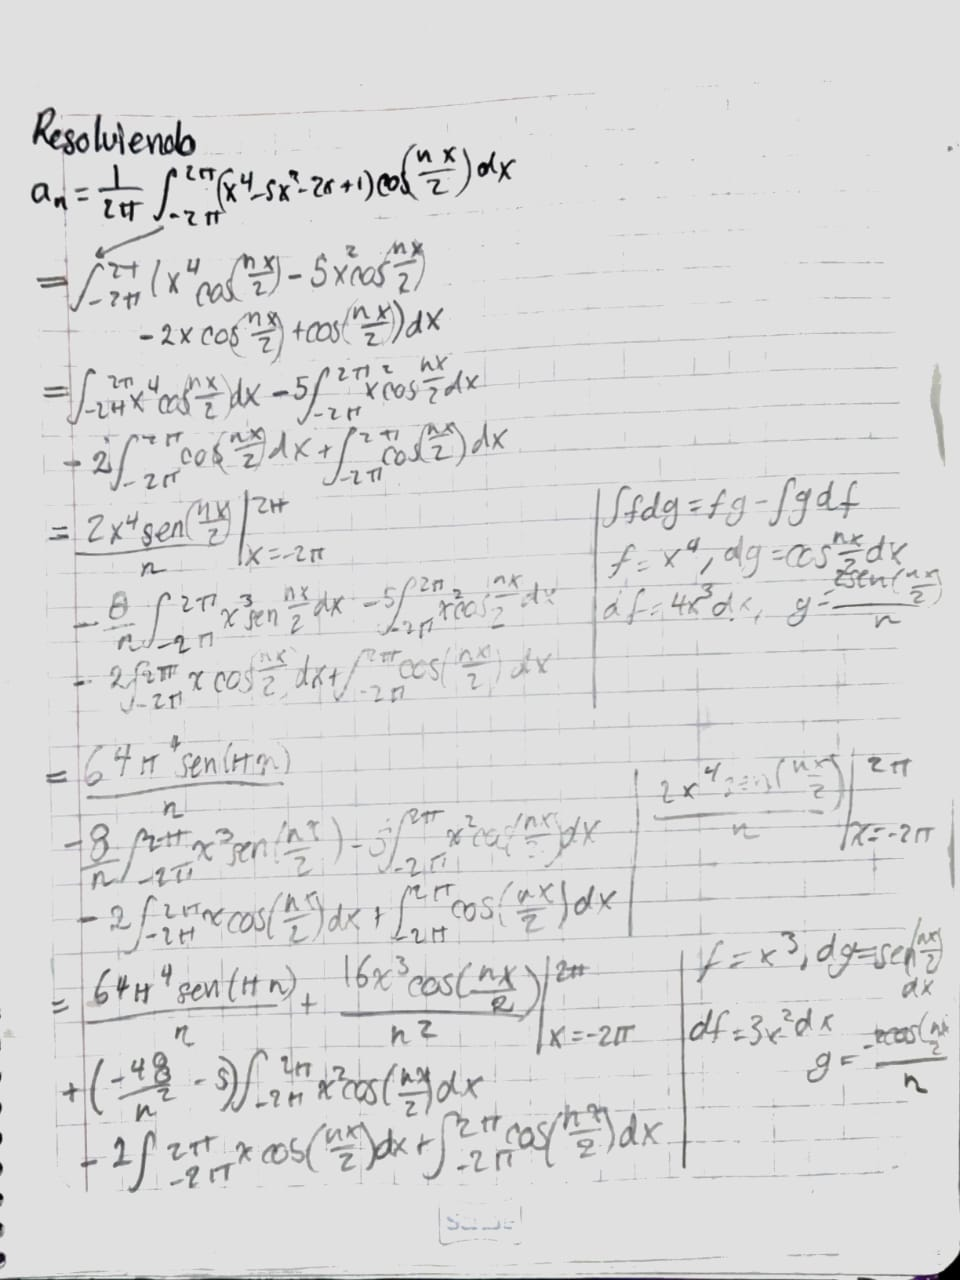
\includegraphics[width=3.12761in,height=4.17188in]{media/image31.jpg}
	\caption{Imagen C2. Primero determinaremos la forma cerrada del término \(a_n\).}
\end{figure}

\begin{figure}[H]
	\centering
	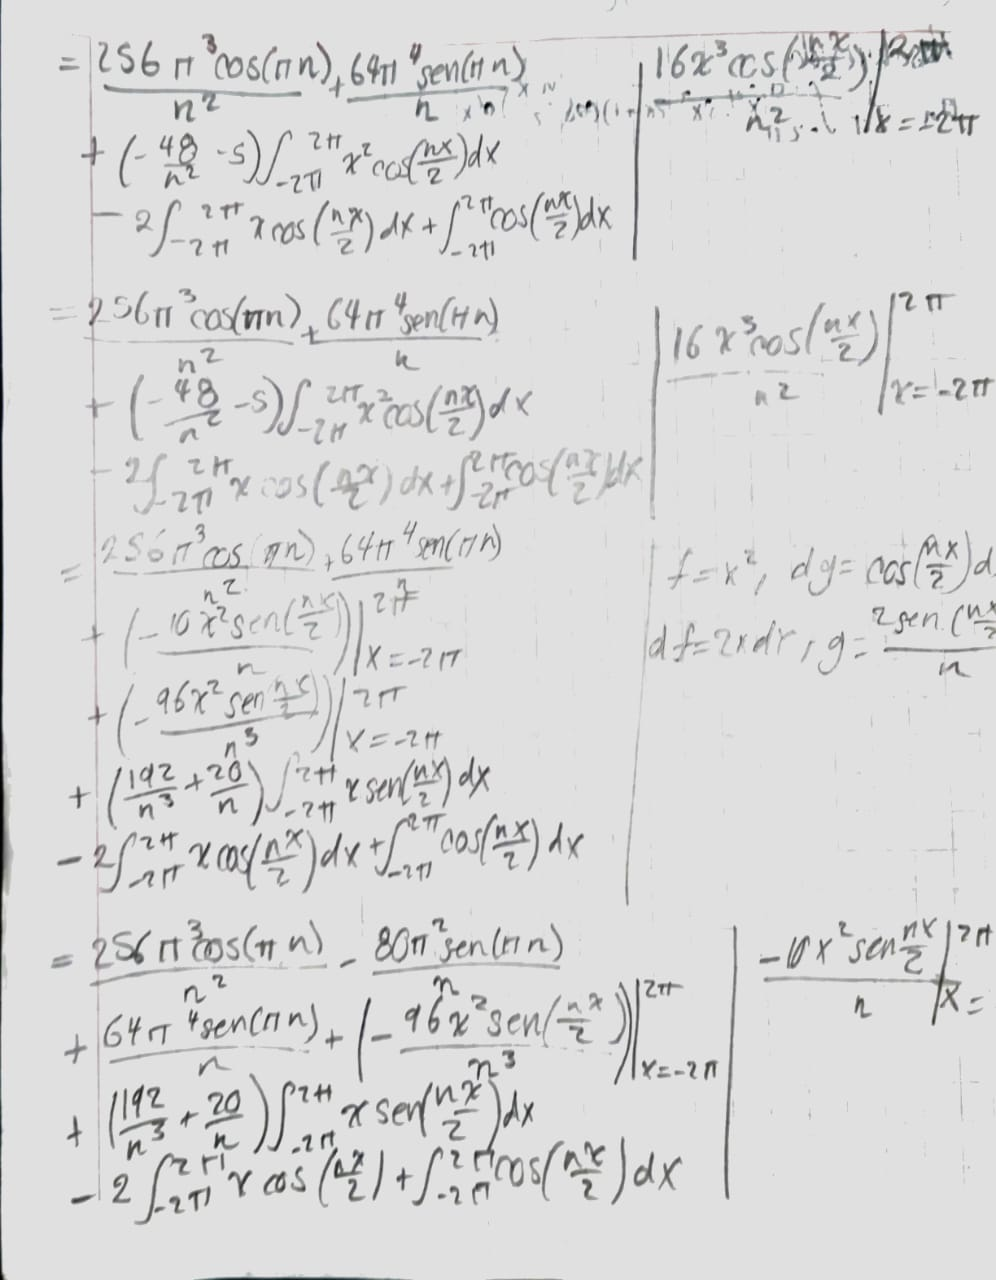
\includegraphics[width=2.78659in,height=3.57813in]{media/image34.jpg}
	\caption{Imagen C3. Continuación del cálculo \(a_n\).}
\end{figure}

\begin{figure}[H]
	\centering
	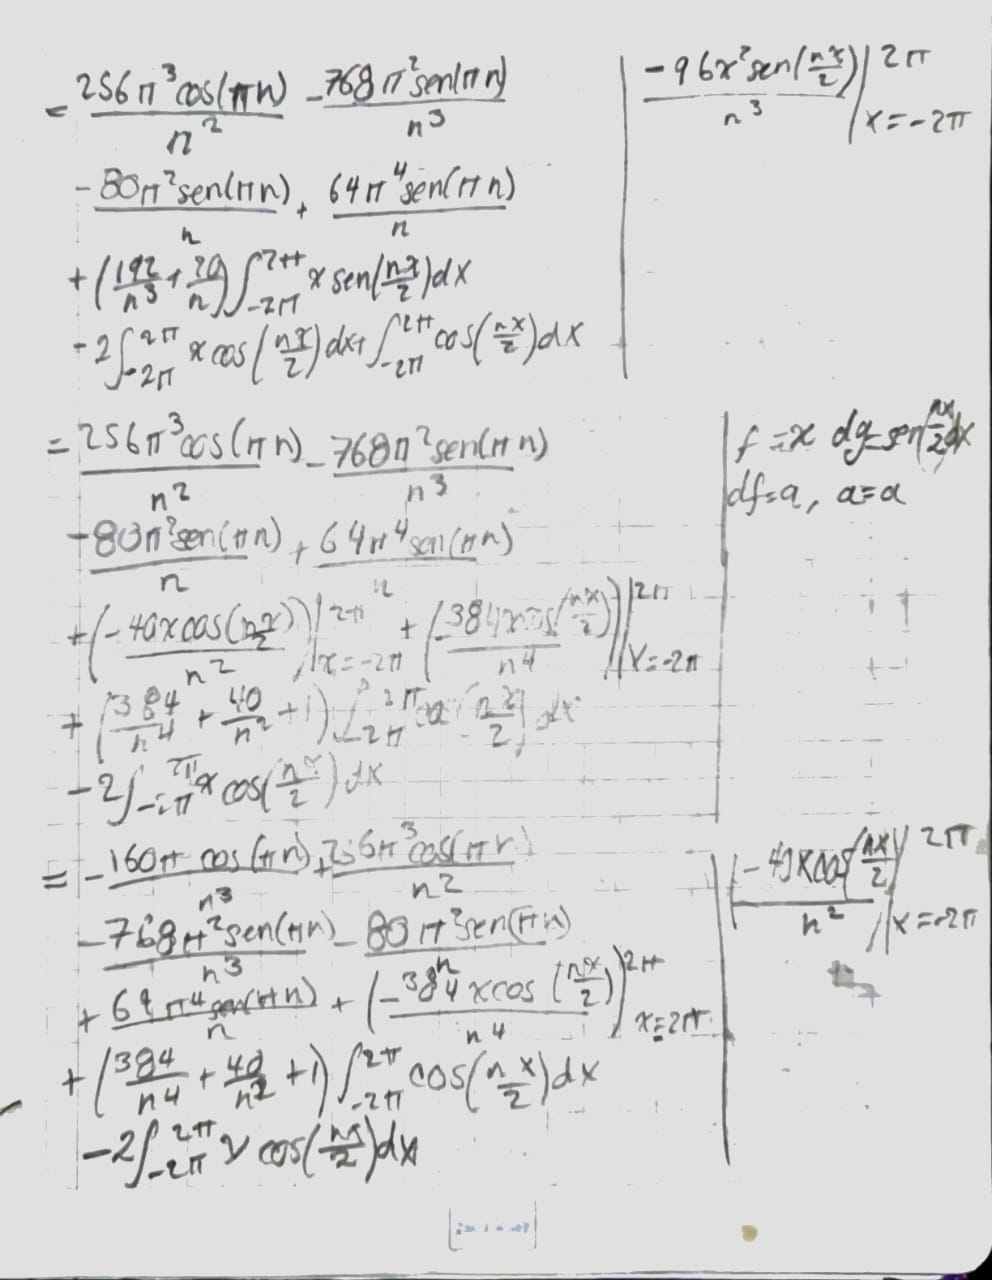
\includegraphics[width=2.84046in,height=3.66146in]{media/image14.jpg}
	\caption{Imagen C4. Continuación cálculo \(a_n\).}
\end{figure}

\begin{figure}[H]
	\centering
	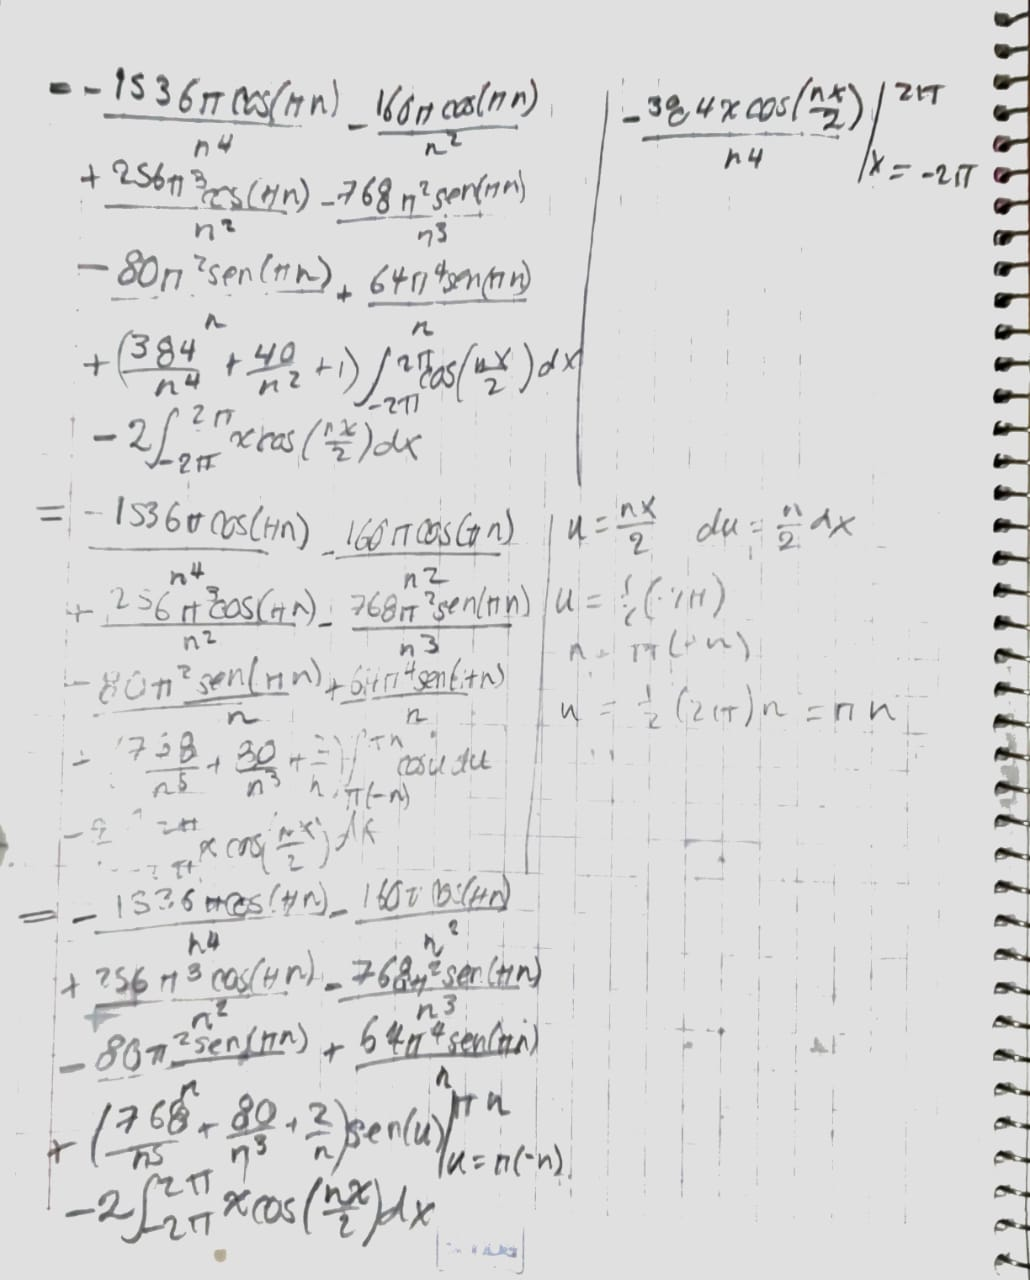
\includegraphics[width=2.66175in,height=3.30729in]{media/image15.jpg}
	\caption{Imagen C5. Continuación cálculo \(a_n\).}
\end{figure}

\begin{figure}[H]
	\centering
	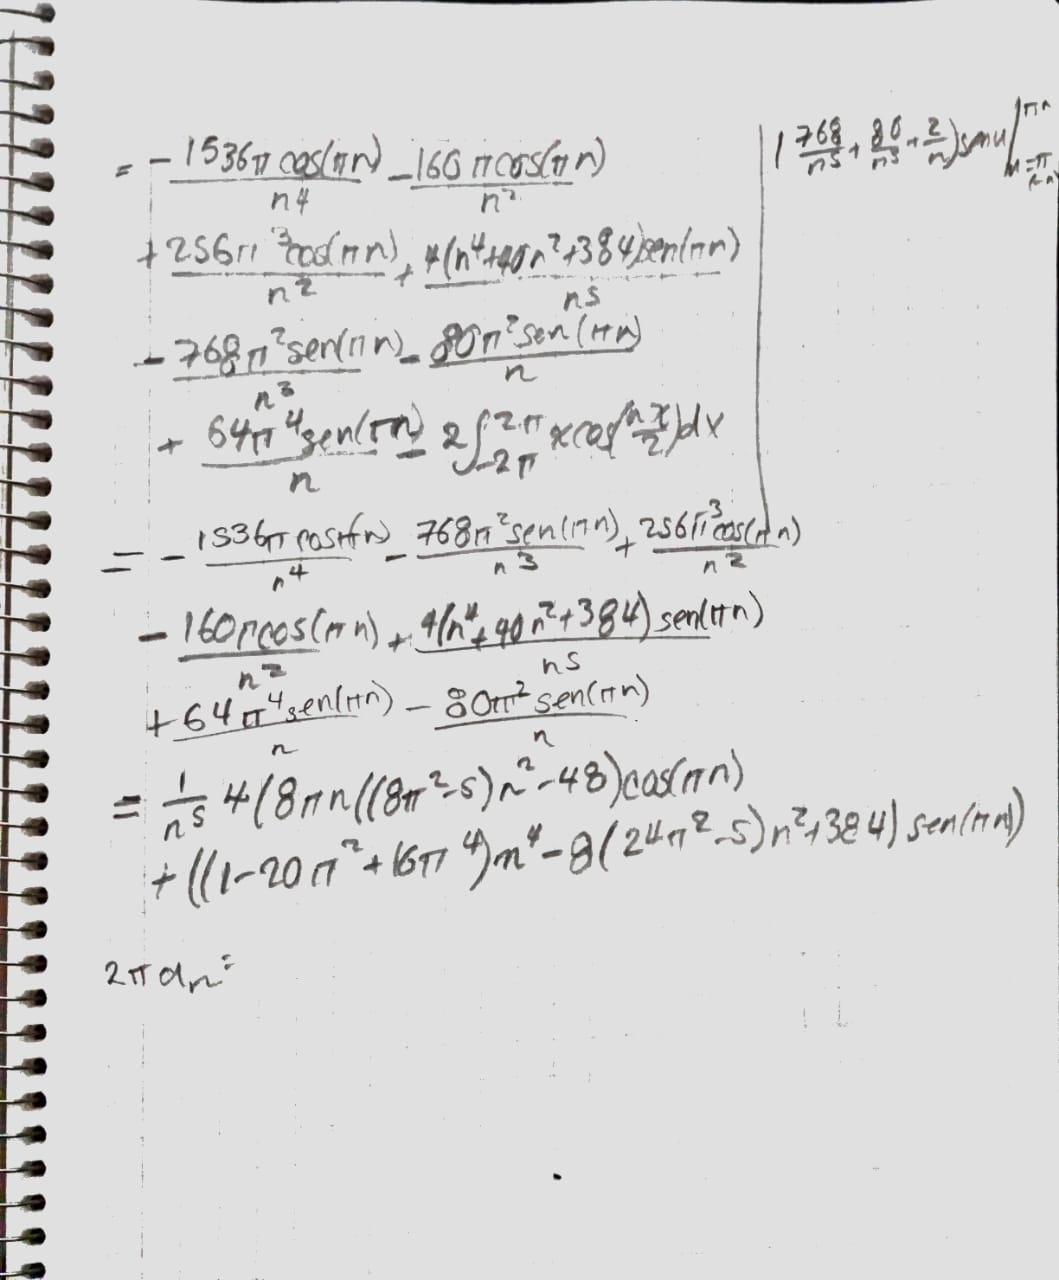
\includegraphics[width=3.09896in,height=3.74243in]{media/image45.jpg}
	\caption{Imagen C6. Finalmente, definimos que el término \(a_n\) es igual a lo que se muestra en la foto.}
\end{figure}

\begin{figure}[H]
	\centering
	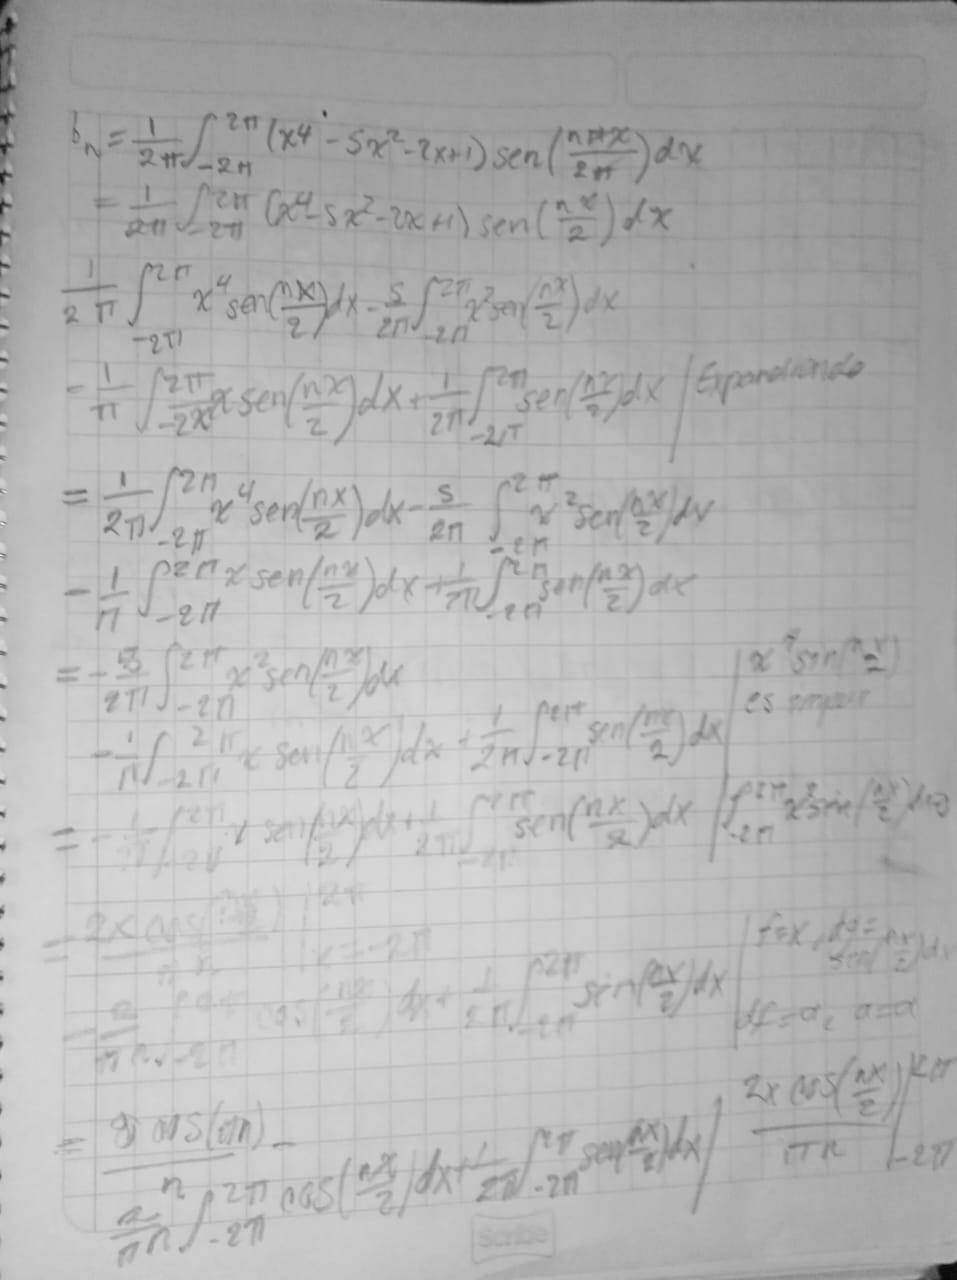
\includegraphics[width=2.6836in,height=3.58854in]{media/image26.jpg}
	\caption{Imagen C7. Continuamos con la determinación del término \(b_n\).}
\end{figure}

\begin{figure}[H]
	\centering
	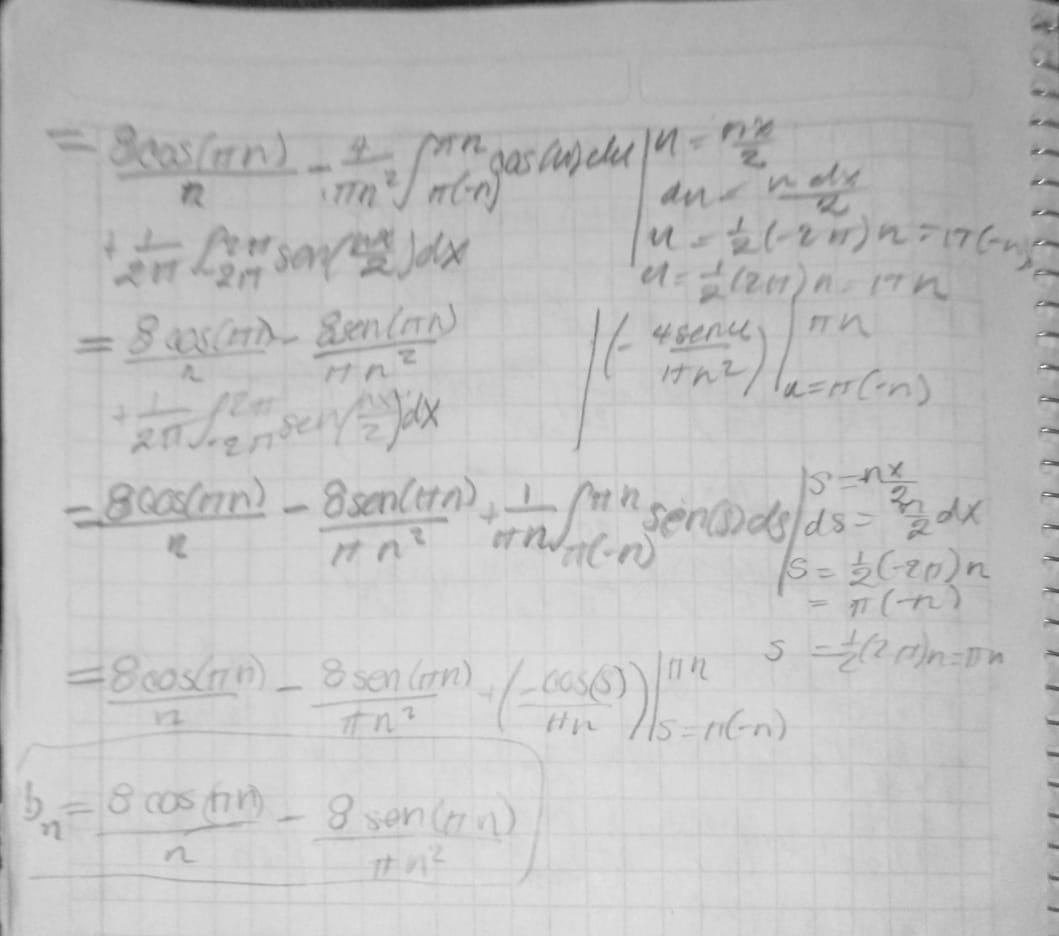
\includegraphics[width=4.00521in,height=3.53949in]{media/image41.jpg}
	\caption{Imagen C8. Y ese es el término \(b_n\) para la serie de Fourier. Sustituímos en la forma de la serie mencionada al principio. Cabe señalar que fue mucho más sencillo calcular \(b_n\) por la propiedad de la función seno de ser impar.}
\end{figure}

\subsection{Oscar Uriel Juárez Tolamatl}

\begin{figure}[H]
	\centering
	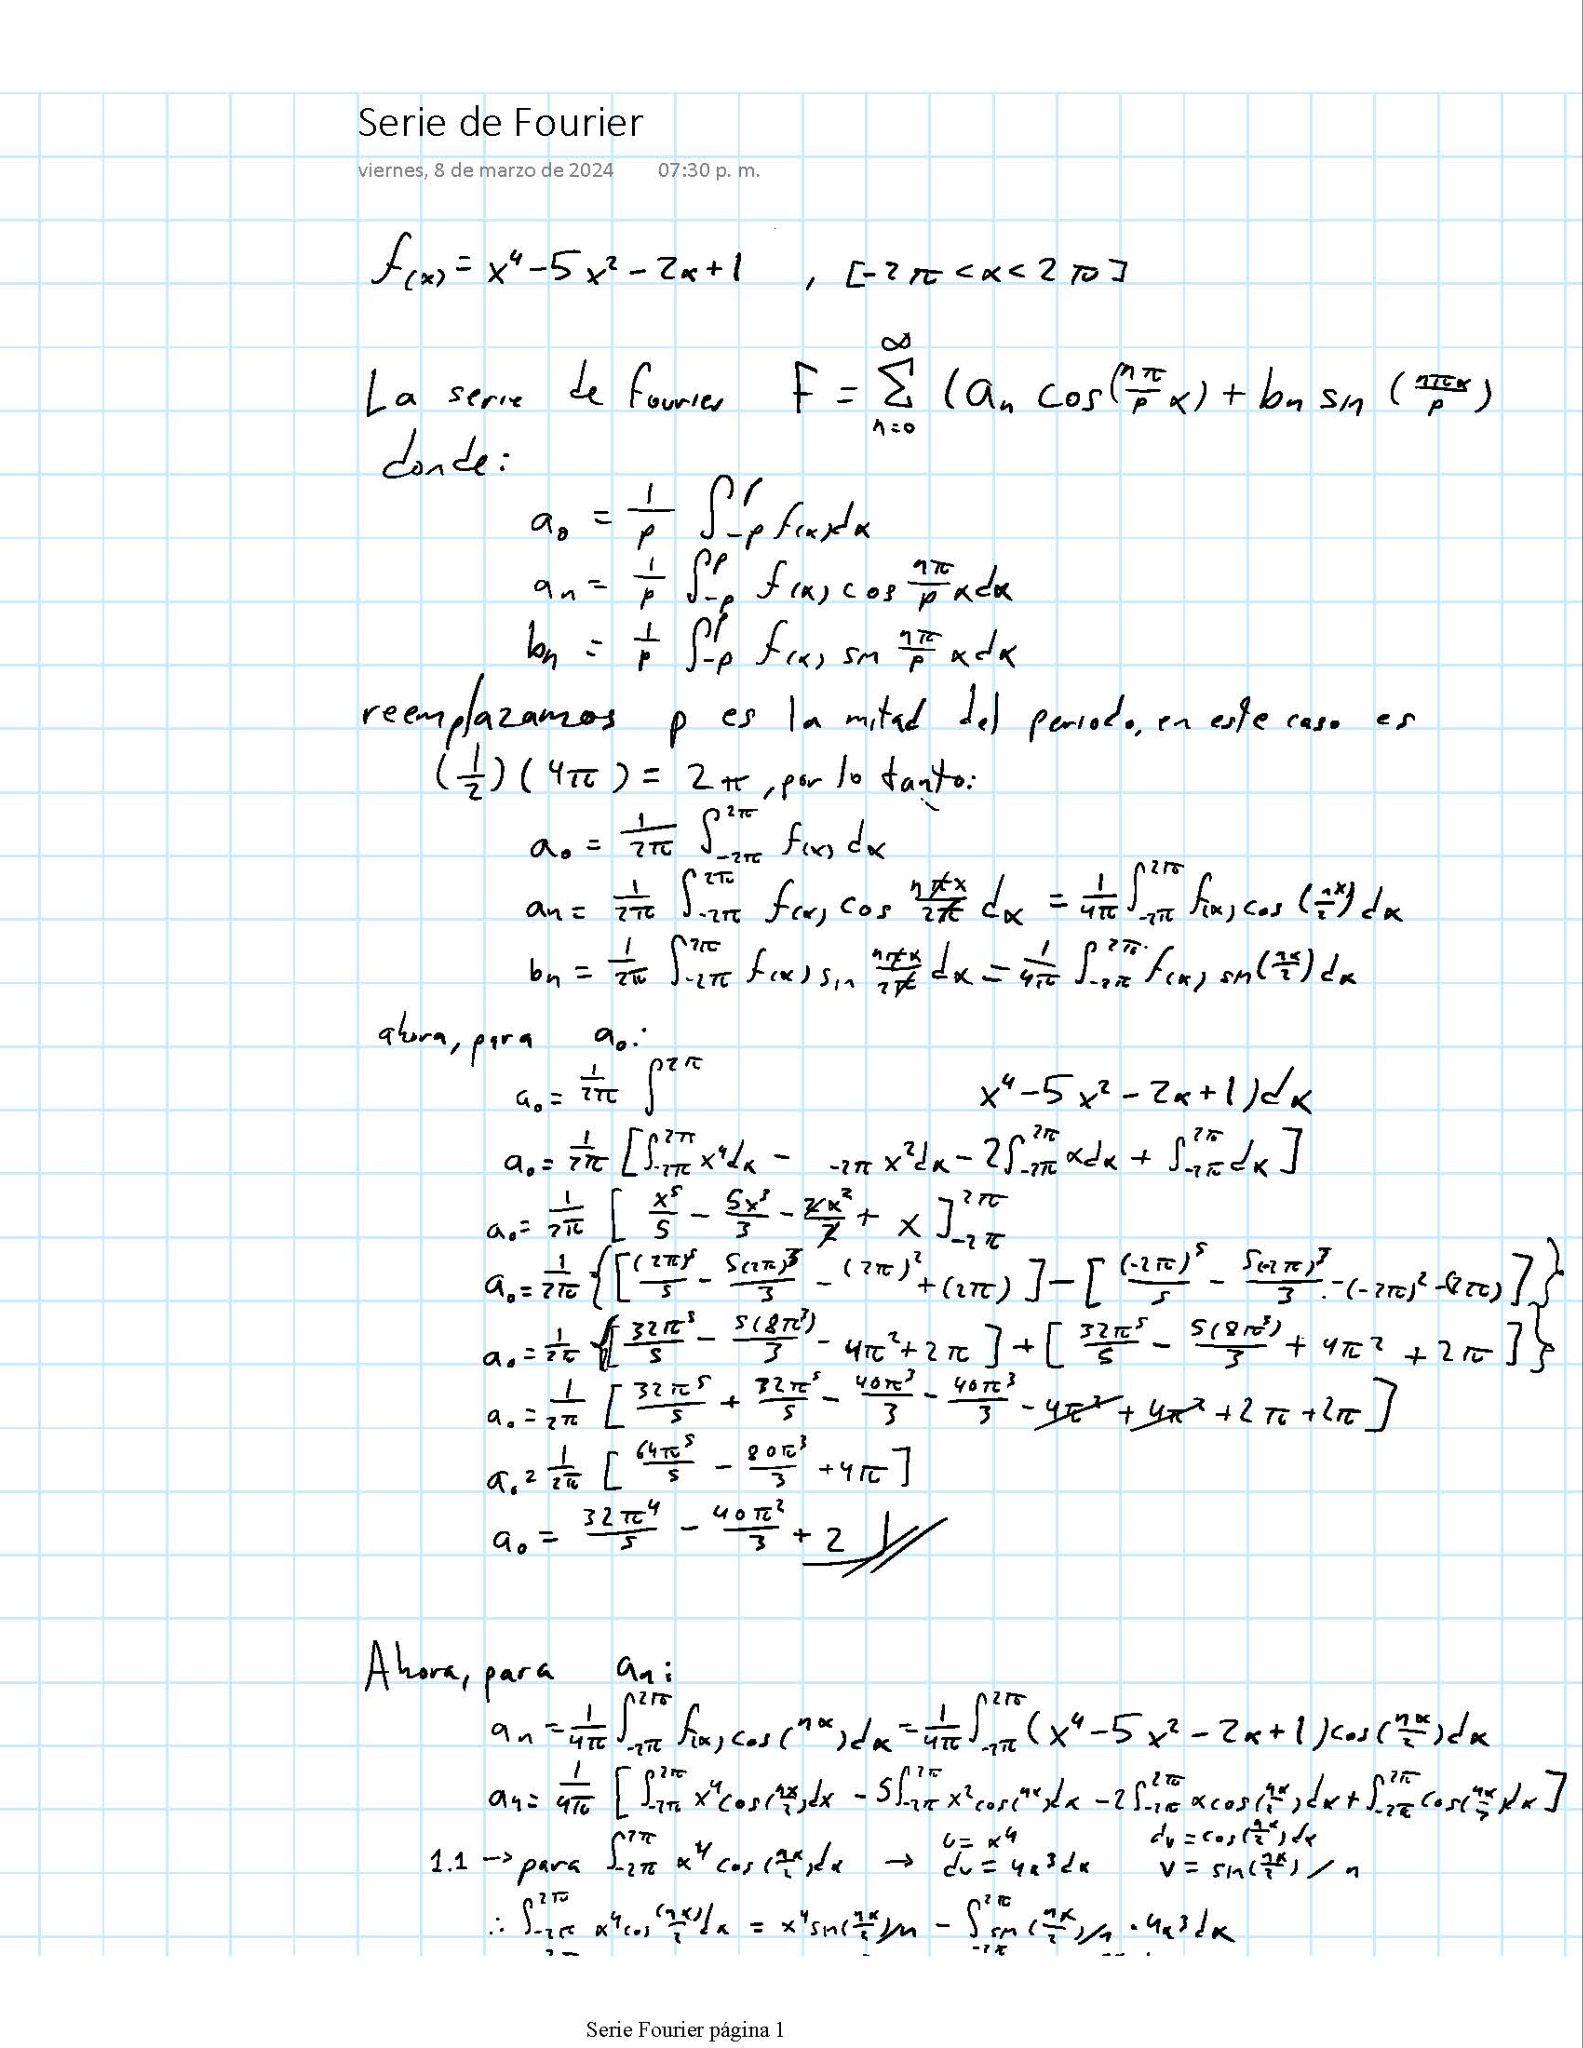
\includegraphics[width=5.93125in,height=7.67516in]{media/image59.jpg}
	\caption{Imagen 1D. Procedimiento de Fourier}
\end{figure}

\begin{figure}[H]
	\centering
	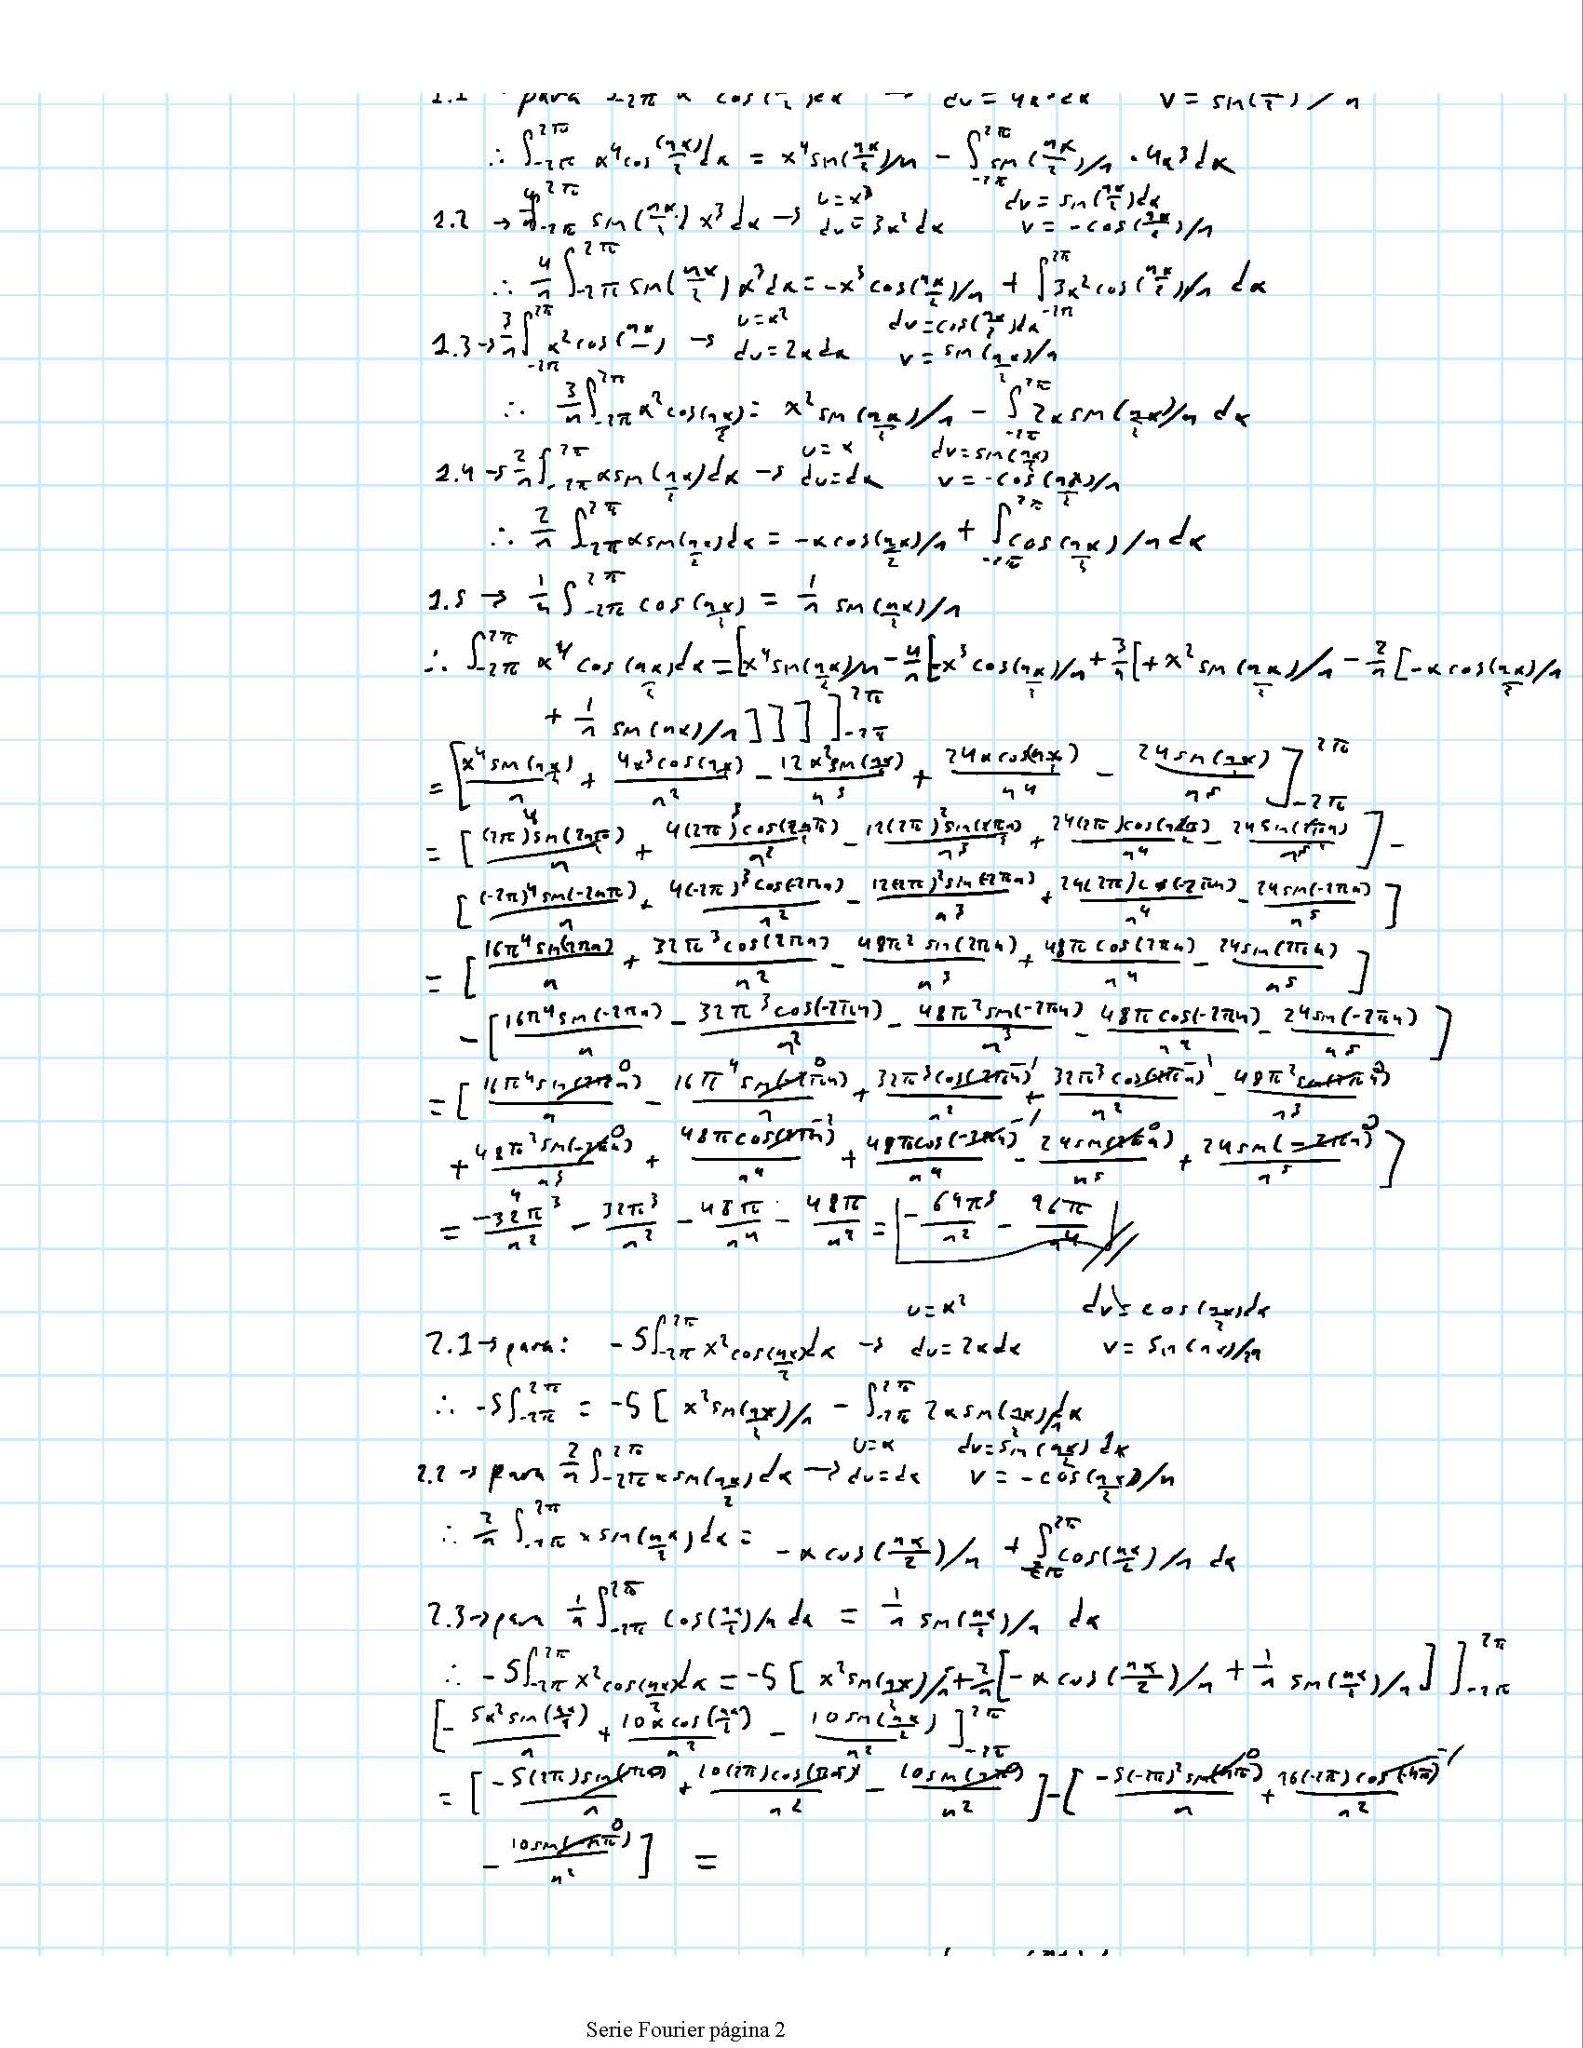
\includegraphics[width=6.26772in,height=8.11111in]{media/image56.jpg}
	\caption{Imagen 2D. Procedimiento de Fourier}
\end{figure}

\begin{figure}[H]
	\centering
	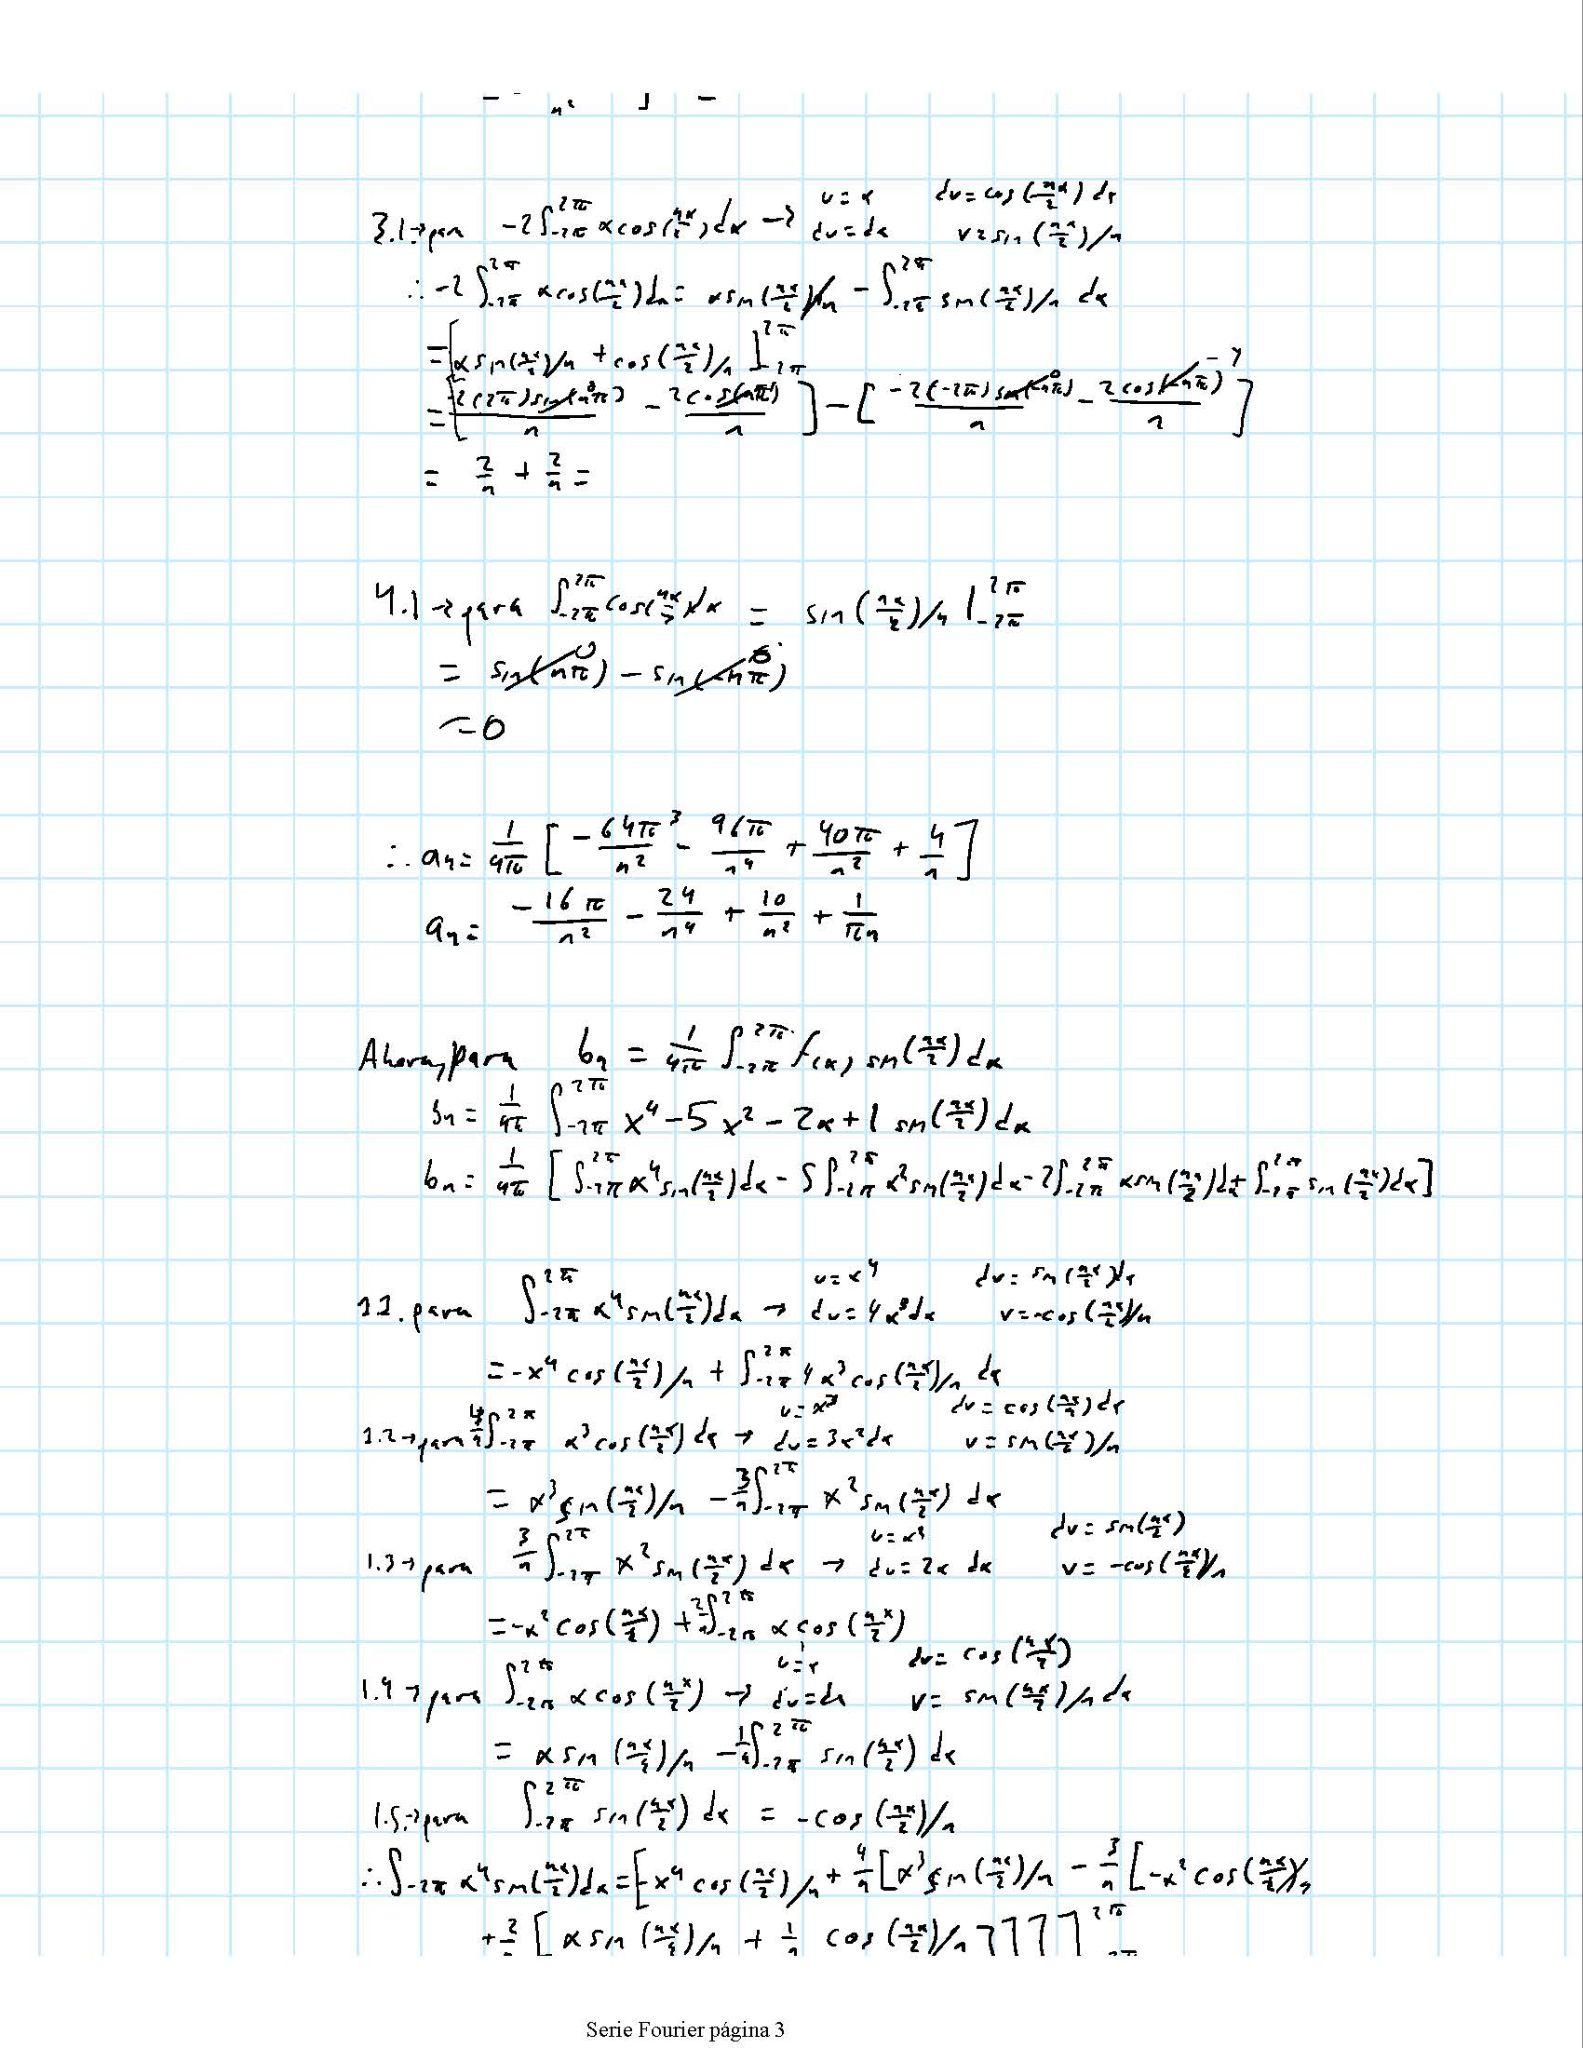
\includegraphics[width=6.26772in,height=8.11111in]{media/image55.jpg}
	\caption{Imagen 3D. Procedimiento de Fourier}
\end{figure}

\begin{figure}[H]
	\centering
	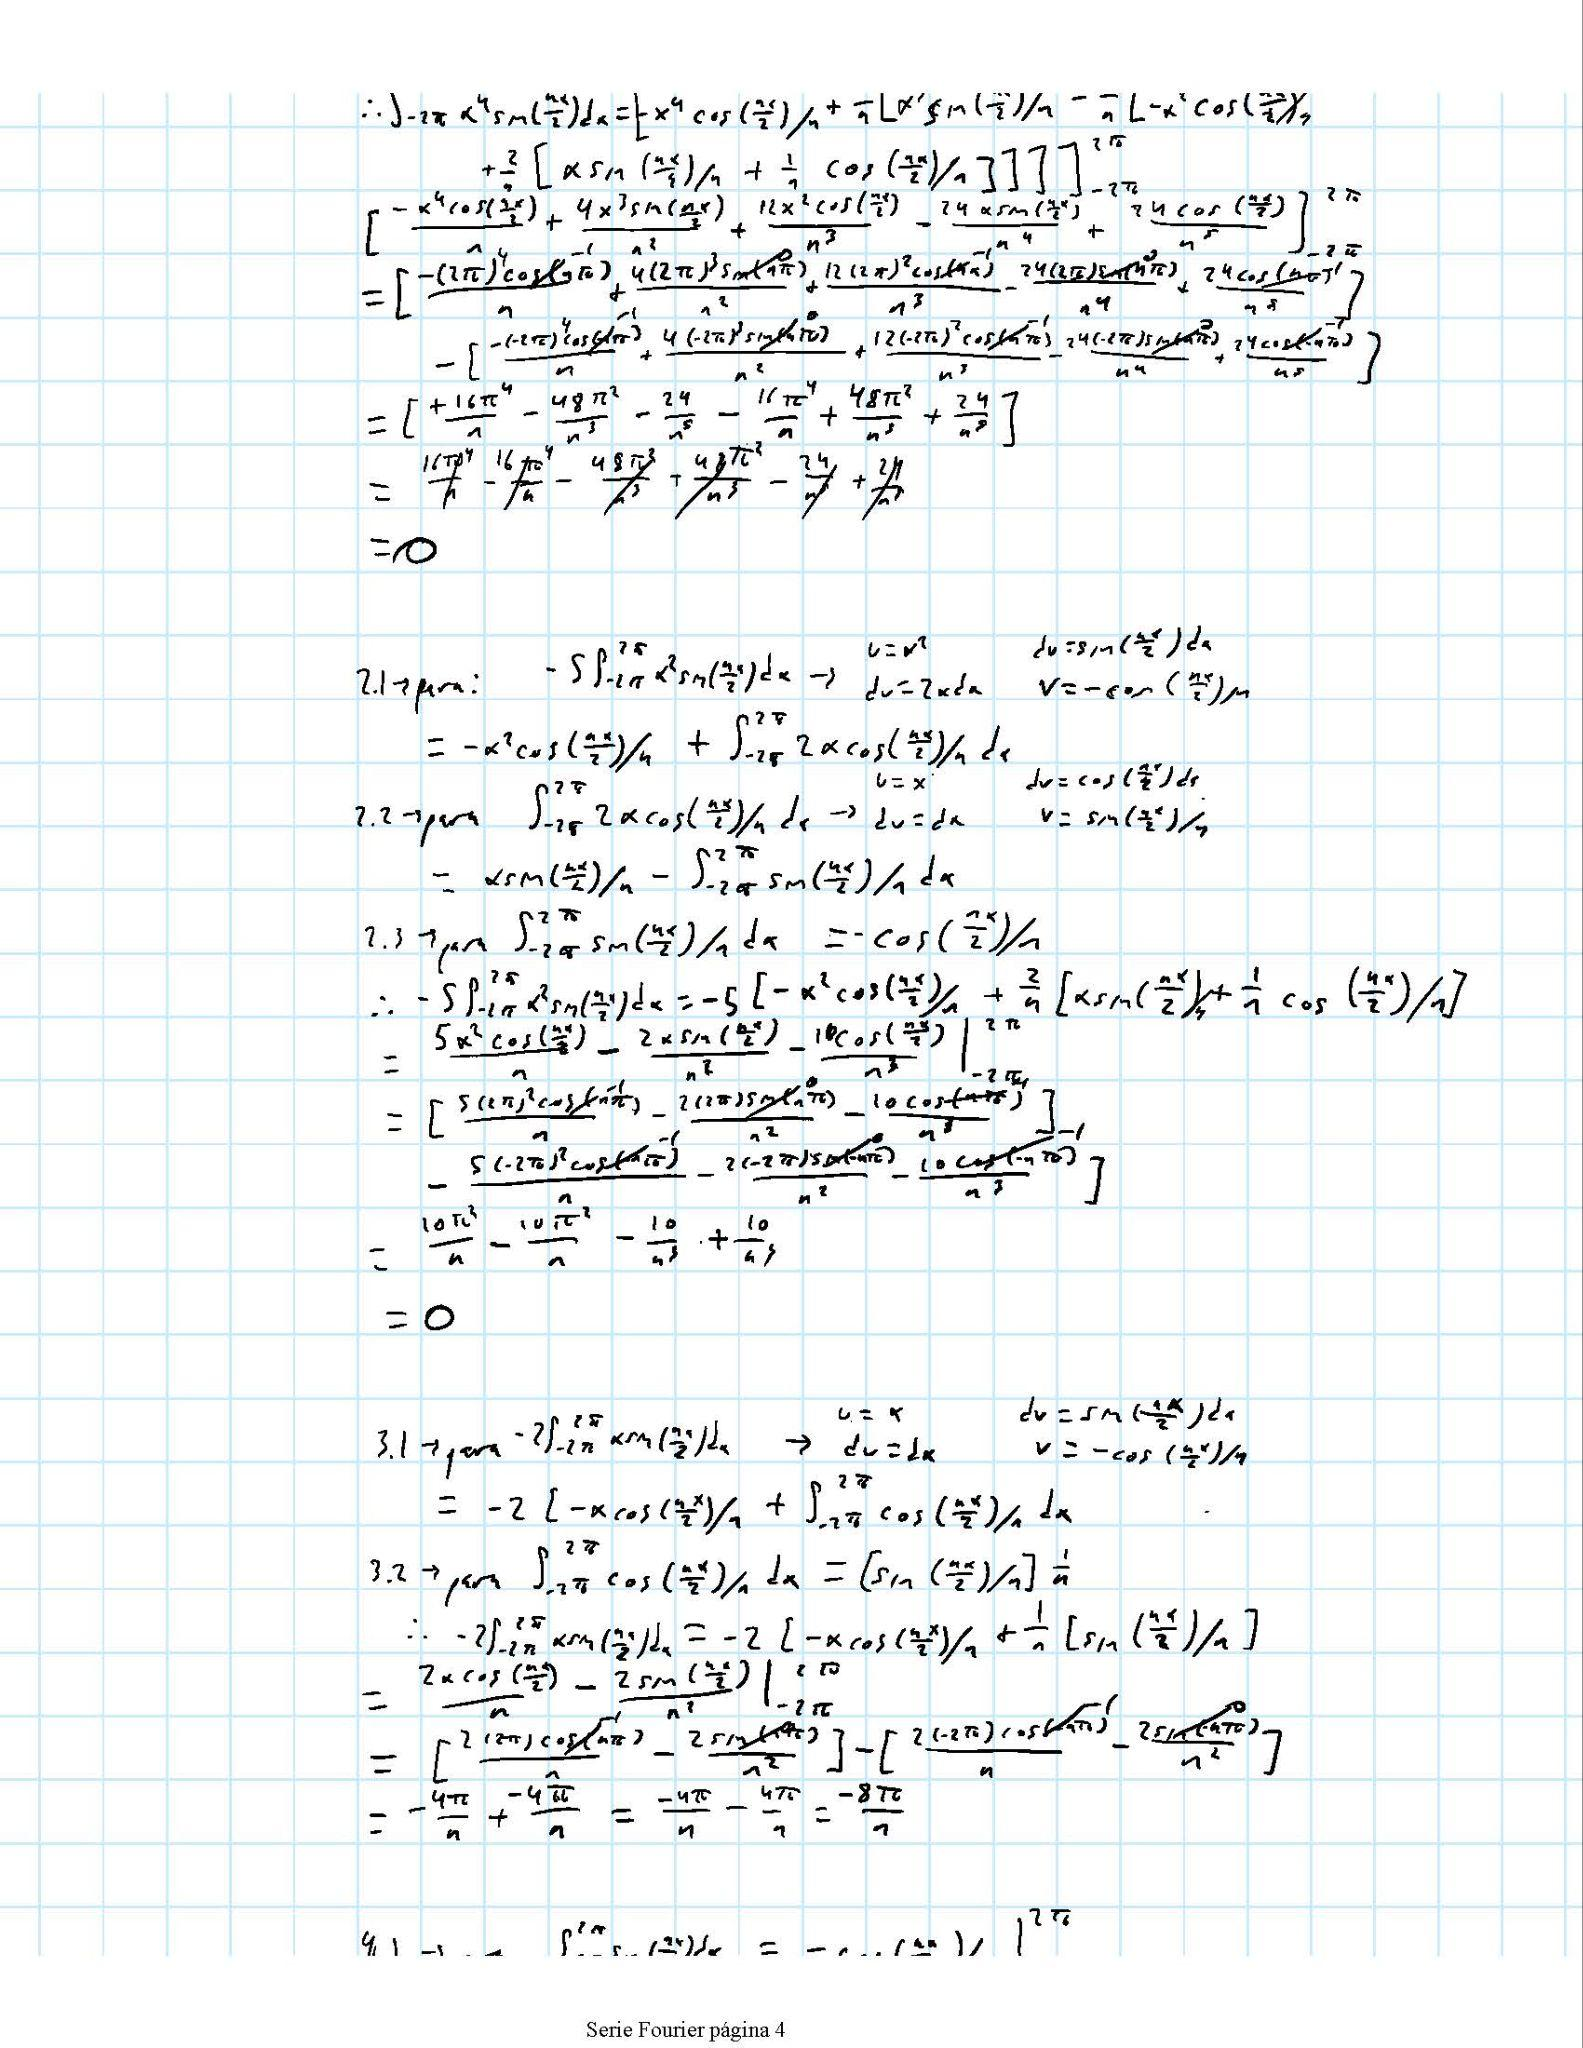
\includegraphics[width=6.26772in,height=8.11111in]{media/image57.jpg}
	\caption{Imagen 4D. Procedimiento de Fourier}
\end{figure}

\begin{figure}[H]
	\centering
	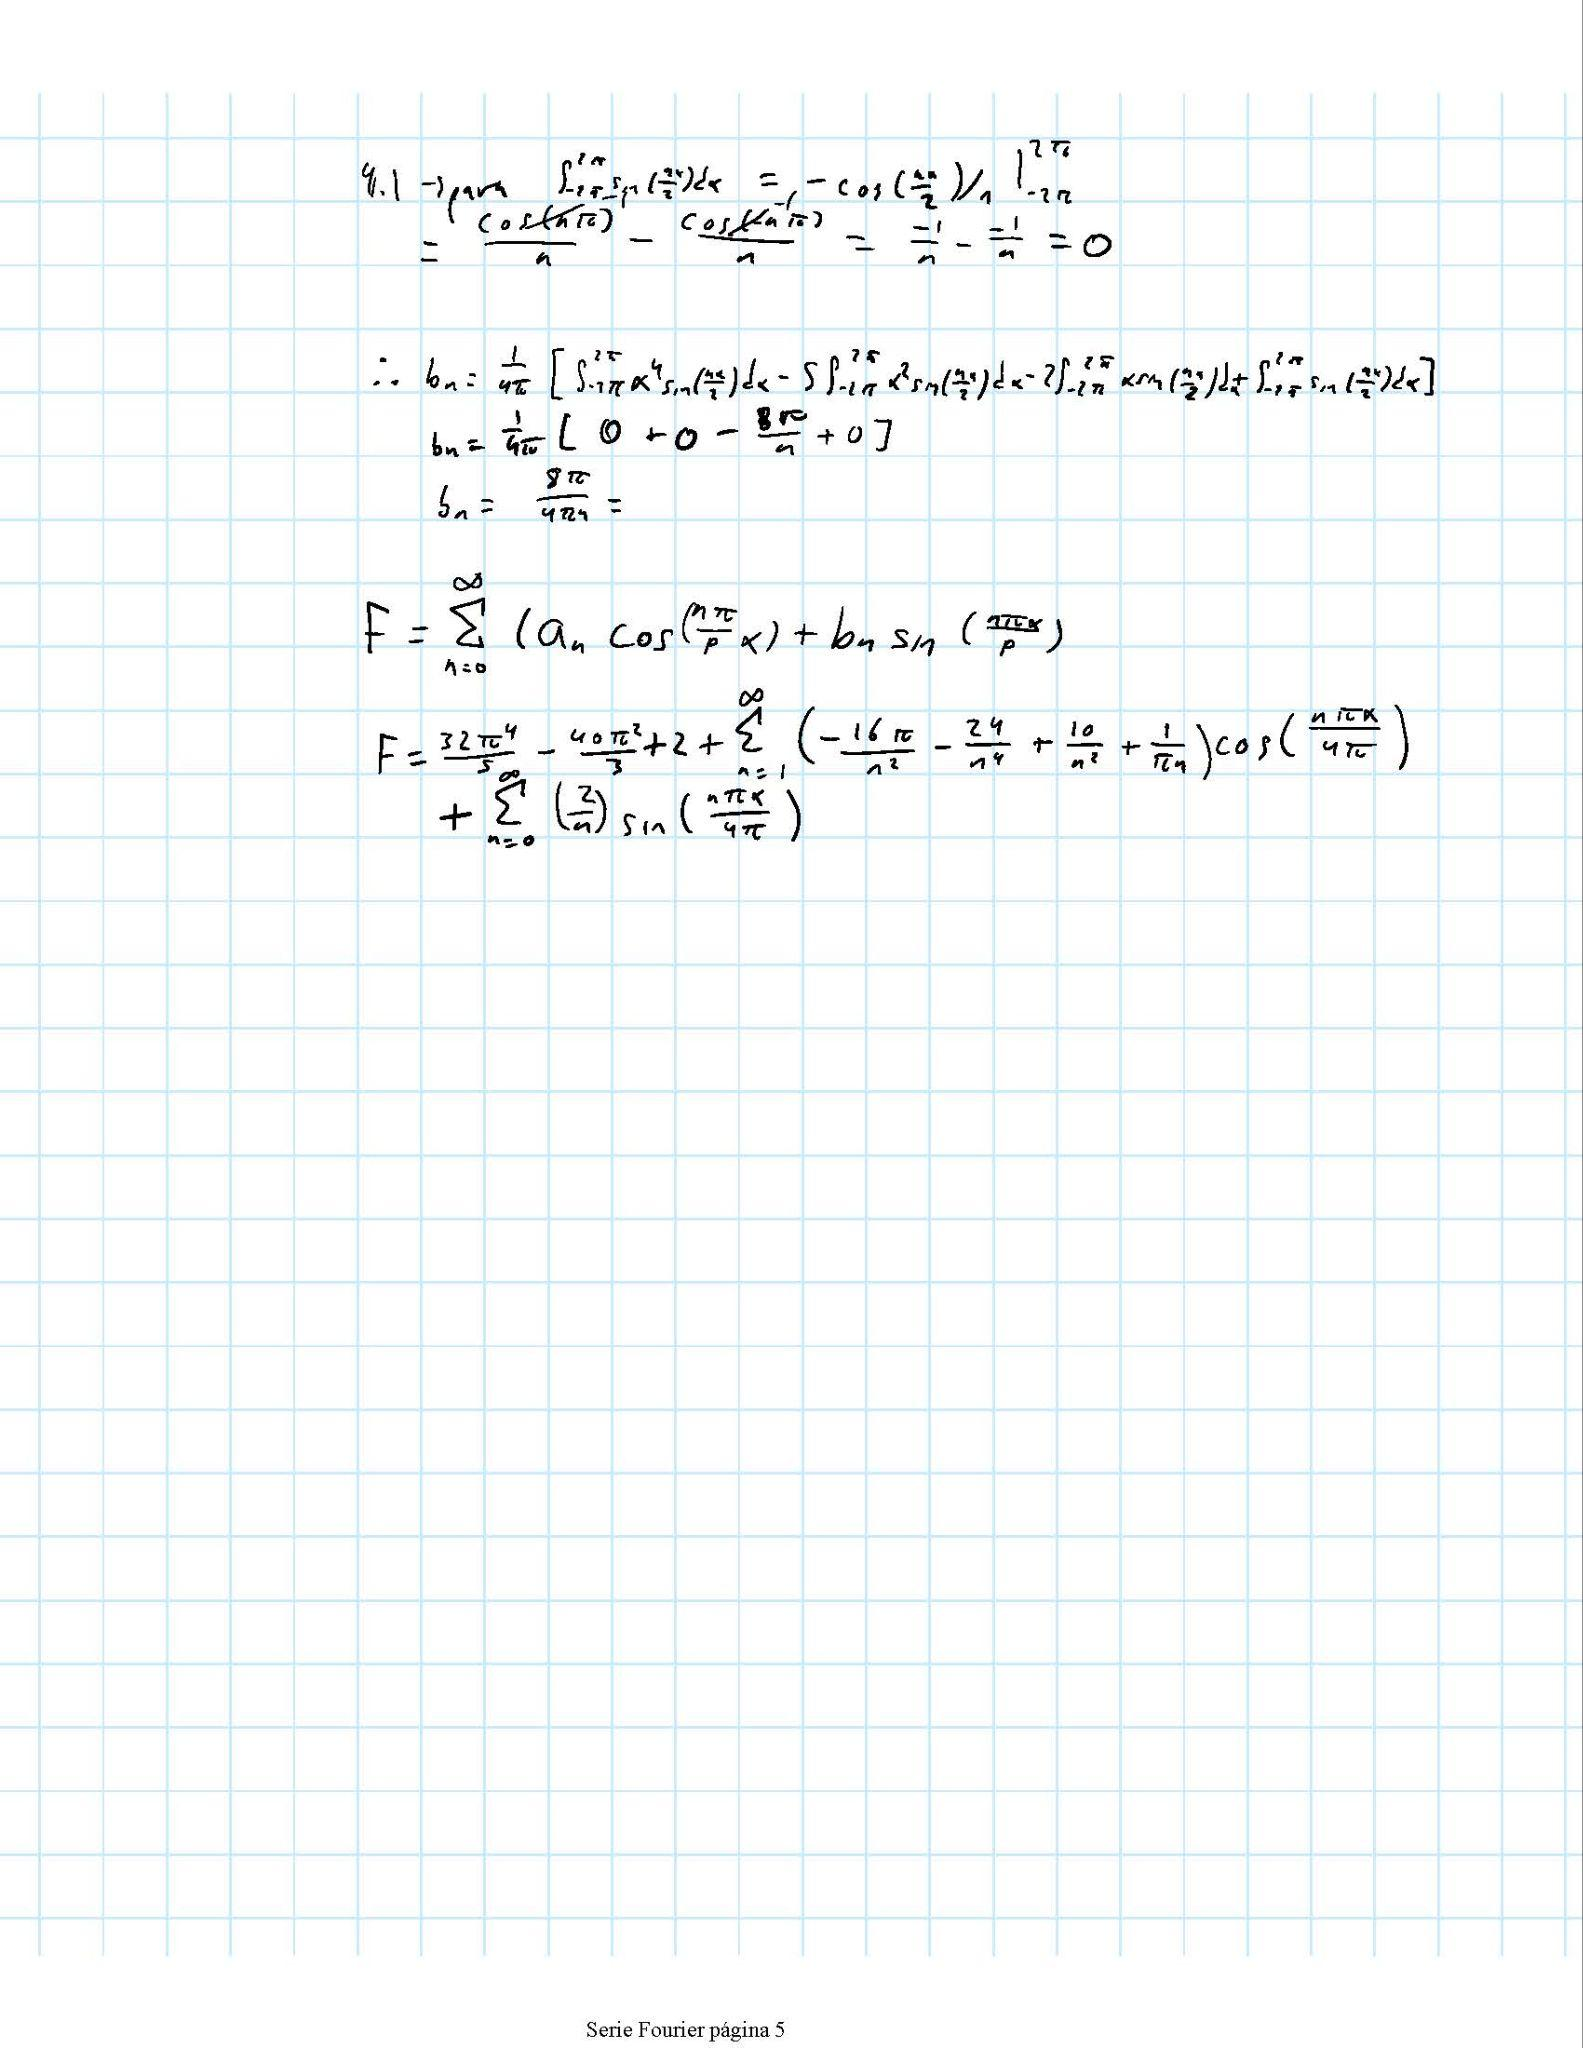
\includegraphics[width=6.26772in,height=8.11111in]{media/image58.jpg}
	\caption{Imagen 5D. Procedimiento de Fourier}
\end{figure}
